\documentclass[a4paper]{article}
\usepackage[T1]{fontenc}			% pacchetto per \chapter
\usepackage[italian]{babel}
\usepackage[italian]{isodate}  		% formato delle date in italiano
\usepackage{graphicx}				% gestione delle immagini
\usepackage{amsfonts}
\usepackage{booktabs}				% tabelle di qualità superiore
\usepackage{amsmath}				% pacchetto matematica
\usepackage{mathtools}				% per sottolineare sotto le equazioni
\usepackage{stmaryrd} 				% per '\llbracket' e '\rrbracket'
\usepackage{amsthm}					% teoremi migliorati
\usepackage{enumitem}				% gestione delle liste
\usepackage{pifont}					% pacchetto con elenchi carini
\usepackage{enumitem}				% pacchetto per elenchi con lettere dell'alfabeto
\usepackage{cancel}					% per cancellare delle espressioni matematiche



\usepackage[x11names]{xcolor}		% pacchetto colori RGB
% Link ipertestuali per l'indice
\usepackage{xcolor}
\usepackage[linkcolor=black, citecolor=blue, urlcolor=cyan]{hyperref}
\hypersetup{
	colorlinks=true
}

\usepackage{tikz}
\newcommand{\MyTikzmark}[2]{%
	\tikz[overlay,remember picture,baseline] \node [anchor=base] (#1) {#2};%
}
\newcommand{\DrawVLine}[3][]{%
	\begin{tikzpicture}[overlay,remember picture]
		\draw[shorten <=0.3ex, #1] (#2.north) -- (#3.south);
	\end{tikzpicture}
}
\newcommand{\DrawHLine}[3][]{%
	\begin{tikzpicture}[overlay,remember picture]
		\draw[shorten <=0.2em, #1] (#2.west) -- (#3.east);
	\end{tikzpicture}
}


%\usepackage{showframe}				% visualizzazione bordi
%\usepackage{showkeys}				% visualizzazione etichetta

\newtheorem{theorem}{\textcolor{Red3}{\underline{Teorema}}}
\newtheorem{lemma}{Lemma}
\renewcommand{\qedsymbol}{QED}
\newcommand{\exec}[1]{\llbracket #1\:\rrbracket}
\newcommand{\dquotes}[1]{``#1''}
\newcommand{\longline}{\noindent\rule{\textwidth}{0.4pt}}
\newcommand{\circledtext}[1]{\raisebox{.5pt}{\textcircled{\raisebox{-.9pt}{#1}}}}

\newenvironment{rowequmat}[1]{\left(\array{@{}#1@{}}}{\endarray\right)}
\newenvironment{rowequmatbra}[1]{\left[\array{@{}#1@{}}}{\endarray\right]}

\begin{document}
	\author{VR443470}
	\title{Esercitazioni Algebra Lineare}
	\date{\printdayoff\today}
	\maketitle
	
	\newpage
	
	% indice
	\tableofcontents
	
	\newpage
	
	\section{Basi}
	
	\subsection{Somma e trasposte}
	
	I classici esercizi di Algebra Lineare prevedono varie operazioni sulle matrici. Partendo dalle basi, si introducono le operazioni di somma e trasposizione.\newline
	
	\noindent
	Date $3$ matrici $A, B, C$:
	\begin{equation*}
		A = \begin{bmatrix}
			   1 & -i & 3 \\
			-2+i &  5 & i2
		\end{bmatrix} \hspace{2em}
		B = \begin{bmatrix}
			3i	& 2		\\
			4	& -i 	\\
			2-i	& -1
		\end{bmatrix} \hspace{2em}
		C = \begin{bmatrix}
			-2	& 3i	& 2-i	\\
			4i	& 1		& 0
		\end{bmatrix}
	\end{equation*}
	La \textcolor{Red3}{prima operazione} da eseguire è la classificazione delle matrici. In questo caso, le matrici hanno le seguenti dimensioni:
	\begin{equation*}
		A\in\mathbb{M}_{2\times3} \hspace{2em} B\in\mathbb{M}_{3\times2} \hspace{2em} C\in\mathbb{M}_{2\times3}
	\end{equation*}
	La \textcolor{Red3}{seconda operazione} da eseguire è controllare se è possibile eseguire l'operazione richiesta dall'esercizio. In questo caso, viene chiesta la somma. Per eseguire quest'ultima (vale lo stesso per la sottrazione), le dimensioni delle matrici devono essere tutte \textbf{identiche}. Dato che in questo caso la matrice $B \left(3\times2\right)$ differisce di dimensione rispetto alle due matrici $A,C \left(2\times3\right)$, è necessario fare qualcosa per eseguire l'operazione di somma.\newline
	
	\noindent
	Dato che è ancora l'inizio, non verranno effettuate manipolazioni complesse. Quindi, si supponga di eseguire questa operazione di somma/sottrazione:
	\begin{equation*}
		2A^{T} - 4\overline{B} + 3C^{T}
	\end{equation*}
	Prima di eseguire l'operazione, si ottengono le relative matrici coniugate e trasposte. L'operazione di \textbf{coniugazione} è eseguibile cambiando i segni ai valori complessi (quindi alle $i$). Invece, l'operazione di \textbf{trasposizione} ($T$) inverte le colonne e le righe di una matrice. I risultati sono:
	\begin{equation*}
		\begin{array}{lllllllll}
			A & = \begin{bmatrix}
				1 	& -i	& 3	\\
				-2+i&  5 	& i2
			\end{bmatrix} &
			A^{T} & = \begin{bmatrix}
				1	& -2+i	\\
				-i	& 5		\\
				3	& i2
			\end{bmatrix} &
			2A^{T} & = \begin{bmatrix}
				2	& -4+2i	\\
				-2i	& 10	\\
				6	& 4i
			\end{bmatrix} \\
			%%%%%%%%%%%%%%%%%%%%%%%%%%%%%%%%%%%%%%%%
			&&&&& \\
			%%%%%%%%%%%%%%%%%%%%%%%%%%%%%%%%%%%%%%%%
			B & = \begin{bmatrix}
				3i	& 2		\\
				4	& -i 	\\
				2-i	& -1
			\end{bmatrix} &
			\overline{B} & = \begin{bmatrix}
				-3i	& 2		\\
				4	& i		\\
				2+i	& -1
			\end{bmatrix} &
			4\overline{B} & = \begin{bmatrix}
				-12i	& 8		\\
				16		& 4i	\\
				8+4i	& -4
			\end{bmatrix} \\
			%%%%%%%%%%%%%%%%%%%%%%%%%%%%%%%%%%%%%%%%
			&&&&& \\
			%%%%%%%%%%%%%%%%%%%%%%%%%%%%%%%%%%%%%%%%
			C & = \begin{bmatrix}
				-2	& 3i	& 2-i	\\
				4i	& 1		& 0
			\end{bmatrix} &
			C^{T} & = \begin{bmatrix}
				-2	& 4i	\\
				3i	& 1		\\
				2-i	& 0
			\end{bmatrix} &
			3C^{T} & = \begin{bmatrix}
				-6	& 12i	\\
				9i	& 3		\\
				6-3i& 0
			\end{bmatrix}
		\end{array}
	\end{equation*}\newpage
	Adesso è possibile eseguire la sottrazione tra $\alpha = 2A^{T} - 4\overline{B}$ e successivamente la somma tra $\alpha + 3C^{T}$:
	\begin{equation*}
		\alpha = 2A^{T} - 4\overline{B} = \begin{bmatrix}
			2	& -4+2i	\\
			-2i	& 10	\\
			6	& 4i
		\end{bmatrix} - \begin{bmatrix}
			-12i	& 8		\\
			16		& 4i	\\
			8+4i	& -4
		\end{bmatrix} = \begin{bmatrix}
			2+12i	& 12+2i		\\
			-16-2i	& 10-4i		\\
			1-4i	& 4+4i
		\end{bmatrix}
	\end{equation*}
	Si esegue la somma:
	\begin{equation*}
		\alpha + 3C^{T} = \begin{bmatrix}
			2+12i	& 12+2i		\\
			-16-2i	& 10-4i		\\
			1-4i	& 4+4i
		\end{bmatrix} + \begin{bmatrix}
			-6	& 12i	\\
			9i	& 3		\\
			6-3i& 0
		\end{bmatrix} = \begin{bmatrix}
			-4+12i	& -12+14i	\\
			-16+7i	& 13-4i		\\
			7-7i	& 4+4i
		\end{bmatrix}
	\end{equation*}\newpage

	\subsection{(Anti-)Hermitiane e (anti-)simmetriche}
	
	Diamo alcune definizioni per capire come fare gli esercizi:
	\begin{itemize}
		\item È possibile abbreviare letteralmente le operazioni di trasposizione e coniugazione scrivendo \textbf{trasposta-coniugata};
		
		\item Una matrice viene detta \textcolor{Red3}{\textbf{hermitiana}} quando la matrice originaria è uguale alla sua trasposta-coniugata:
		\begin{equation*}
			\overline{\left(A^{T}\right)} = \left(\overline{A}\right)^{T} = A \Longrightarrow A^{H}
		\end{equation*}
		
		\item Una matrice viene detta \textcolor{Red3}{\textbf{anti-hermitiana}} quando la matrice trasposta-coniugata corrisponde alla matrice originaria ma cambiata di segno:
		\begin{equation*}
			\overline{\left(A^{T}\right)} = \left(\overline{A}\right)^{T} = -A \Longrightarrow \text{ anti-hermitiana}
		\end{equation*}
		
		\item Una matrice viene detta \textcolor{Red3}{\textbf{simmetrica}} quando la matrice originaria è uguale alla sua trasposta:
		\begin{equation*}
			A = A^{T} \Longrightarrow \text{ simmetrica}
		\end{equation*}
		
		\item Una matrice viene detta \textcolor{Red3}{\textbf{anti-simmetrica}} quando la sua trasposta corrisponde alla matrice originaria ma cambiata di segno:
		\begin{equation*}
			-A = A^{T} \Longrightarrow \text{ anti-simmetrica}
		\end{equation*}
	\end{itemize}
	Prendendo come \textcolor{Green4}{\textbf{esempio}} le tre matrici $A,B,C$:
	\begin{equation*}
		A = \begin{bmatrix}
			2i 	& 3		\\
			-3	& i
		\end{bmatrix} \hspace{2em}
		B = \begin{bmatrix}
			i 	& 2		\\
			2	& i
		\end{bmatrix} \hspace{2em}
		C = \begin{bmatrix}
			-1 	& i3	\\
			-i3	& 1
		\end{bmatrix}
	\end{equation*}
	Si eseguono le rispettive operazioni di trasposizione e coniugazione:
	\begin{equation*}
		\begin{array}{lllllllll}
			A & = \begin{bmatrix}
				2i 	& 3		\\
				-3	& i
			\end{bmatrix} &
			A^{T} & = \begin{bmatrix}
				2i	& -3	\\
				3	& i
			\end{bmatrix} &
			\overline{A^{T}} & = \begin{bmatrix}
				-2i	& -3	\\
				3	& -i
			\end{bmatrix} \\
			%%%%%%%%%%%%%%%%%%%%%%%%%%%%%%%%%%%%%%%%
			&&&&& \\
			%%%%%%%%%%%%%%%%%%%%%%%%%%%%%%%%%%%%%%%%
			B & = \begin{bmatrix}
				i 	& 2		\\
				2	& i
			\end{bmatrix} &
			B^{T} & = \begin{bmatrix}
				i	& 2		\\
				2	& i
			\end{bmatrix} &
			\overline{B^{T}} & = \begin{bmatrix}
				-i	& 2		\\
				2	& -i
			\end{bmatrix} \\
			%%%%%%%%%%%%%%%%%%%%%%%%%%%%%%%%%%%%%%%%
			&&&&& \\
			%%%%%%%%%%%%%%%%%%%%%%%%%%%%%%%%%%%%%%%%
			C & = \begin{bmatrix}
				-1 	& i3	\\
				-i3	& 1
			\end{bmatrix} &
			C^{T} & = \begin{bmatrix}
				-1	& -i3	\\
				i3	& 1
			\end{bmatrix} &
			\overline{C^{T}} & = \begin{bmatrix}
				-1	& i3	\\
				-i3	& 1
			\end{bmatrix}
		\end{array}
	\end{equation*}
	Da questi risultati è possibile notare come $A, B$ \underline{non} siano hermitiane, mentre $C$ lo sia. Inoltre, dalle trasposte è possibile osservare come $A, C$ \underline{non} siano simmetriche, mentre $B$ lo sia. Invece, per verificare l'anti-hermitiana e l'anti-simmetrica, è necessario negare le matrici originarie:
	\begin{equation*}
		-A = \begin{bmatrix}
			-2i	& -3	\\
			3	& -i
		\end{bmatrix} \hspace{2em}
		-B = \begin{bmatrix}
			-i 	& -2	\\
			-2	& -i
		\end{bmatrix} \hspace{2em}
		-C = \begin{bmatrix}
			1 	& -i3	\\
			i3	& -1
		\end{bmatrix}
	\end{equation*}
	Da questi risultati è possibile notare come $B,C$ \underline{non} siano anti-hermitiane, mentre $A$ lo sia. Inoltre, osservando nuovamente le trasposte, è possibile osservare come $A, B$ e $C$ \underline{non} siano anti-simmetriche.\newpage
	
	\subsection{Prodotto tra matrici righe per colonne}
	
	La \textcolor{Red3}{prima operazione} da eseguire per la moltiplicazione tra matrici righe per colonne è la verifica delle righe e delle colonne. Il prodotto tra matrici è ammesso solo se il numero delle colonne del primo operando è uguale al numero delle righe del secondo operando. Per esempio, la seguente operazione è ammessa:
	\begin{equation*}
		A_{m \times n} \cdot B_{n \times l}
	\end{equation*}
	Inoltre, la matrice risultante avrà come dimensione le righe del primo operando e le colonne del secondo. Quindi:
	\begin{equation*}
		C_{m \times l} = A_{m \times n} \cdot B_{n \times l}
	\end{equation*}
	La \textcolor{Red3}{seconda operazione} è la moltiplicazione vera e propria. Per farla, si prende ogni riga del primo operando e si moltiplica per ogni colonna del secondo operando. Dopo la moltiplicazione di una riga per una colonna, si sommano i risultati. Quindi:
	\begin{gather*}
		A_{m,n} = \begin{bmatrix}
			1,1 	& \cdots & 1,n 		\\
			\cdots 	& \cdots & \cdots	\\
			m,1		& \cdots & m,n
		\end{bmatrix} \times
		B_{n,l} = \begin{bmatrix}
			1,1 	& \cdots & 1,l 		\\
			\cdots 	& \cdots & \cdots	\\
			n,1		& \cdots & n,l
		\end{bmatrix} \\
		\\
		C_{1,1} = A_{1,1} \cdot B_{1,1} + \cdots + A_{1,n} \cdot B_{n,1} \\
		\cdots
	\end{gather*}
	Si presenta un \textcolor{Green4}{\textbf{esempio}}. Date due matrici $A,B$:
	\begin{equation*}
		A = \begin{bmatrix}
			1 & 0 &  2 \\
			0 & 3 & -1
		\end{bmatrix} \hspace{2em}
		B = \begin{bmatrix}
			4  	& 1 \\
			-2 	& 2 \\
			0 	& 3
		\end{bmatrix}
	\end{equation*}
	L'operazione di moltiplicazione di righe per colonne è ammessa poiché le righe di $A$ ($2$) sono lo stesso numero delle colonne di $B$ ($2$):
	\begin{equation*}
		C = A \cdot B = \begin{bmatrix}
			4  & 7 \\
			-6 & 3
		\end{bmatrix}
	\end{equation*}
	I calcoli sono banali. Si lasciano qua di seguito i passaggi:
	\begin{equation*}
		\begin{array}{lllllllll}
			C_{1,1} & = & 1 \cdot 4 & + & 0 \cdot -2 & + & 2 \cdot 0 & = & 4	\\
			C_{1,2} & = & 1 \cdot 1 & + & 0 \cdot 2 & + & 2 \cdot 3 & = & 7		\\
			C_{2,1} & = & 0 \cdot 4 & + & 3 \cdot -2 & + & -1 \cdot 0 & = & -6	\\
			C_{2,2} & = & 0 \cdot 1 & + & 3 \cdot 2 & + & -1 \cdot 3 & = & 3
		\end{array}
	\end{equation*}\newpage

	\noindent
	Si presenta un altro \textcolor{Green4}{\textbf{esempio}} ma con i numeri complessi. Date le due matrici $A, B$:
	\begin{equation*}
		A_{2,4} = \begin{bmatrix}
			1+i	& i					& 0		& \overline{3+2i} \\
			-i 	& \overline{-1-3i} 	& 7i	& 6i
		\end{bmatrix} \times
		B_{4,2} = \begin{bmatrix}
			2  				& 4i 	\\
			-3i				& 0 	\\
			\overline{1-i} 	& -2i	\\
			5-i				& \overline{2+i}
		\end{bmatrix}
	\end{equation*}
	Prima di eseguire la moltiplicazione tra righe e colonne si risolvono i coniugati, due nella matrice $A$ e due nella matrice $B$:
	\begin{equation*}
		A_{2,4} = \begin{bmatrix}
			1+i	& i			& 0		& 3-2i \\
			-i 	& -1+3i 	& 7i	& 6i
		\end{bmatrix} \times
		B_{4,2} = \begin{bmatrix}
			2  	& 4i 	\\
			-3i	& 0 	\\
			1+i	& -2i	\\
			5-i	& 2-i
		\end{bmatrix}
	\end{equation*}
	L'operazione di moltiplicazione di righe per colonne è ammessa. Quindi si presenta qui di seguito i calcoli eseguiti (attenzione alle parti immaginarie, si ricorda che $i^{2} = -1$):
	\begin{gather*}
		\begin{array}{llllllllllll}
			C_{1,1} & = & \left(1+i\right) \cdot 2 	& + & i \cdot \left(-3i\right) 		& + & 0 \cdot \left(1+i\right) 	& + & \left(3-2i\right) \cdot \left(5-i\right) 	& = & 18-11i \\
			C_{1,2} & = & \left(1+i\right) \cdot 4i 	& + & i \cdot 0 		& + & 0 \cdot -2i	& + & \left(3-2i\right) \cdot \left(2-i\right)	& = & -3i  \\
			C_{2,1} & = & -i \cdot 2	& + & \left(-1+3i\right) \cdot -3i 	& + & 7i \cdot \left(1+i\right) 	& + & 6i \cdot \left(5-i\right) 		& = & 8 + 38i \\
			C_{2,2} & = & -i \cdot 4i 	& + & \left(-1+3i\right) \cdot 0 	& + & 7i \cdot -2i 	& + & 6i \cdot \left(2-i\right) 		& = & 24 + 12i
		\end{array}\\
		\\
		C = \begin{bmatrix}
			18-11i & -3i \\
			8+38i & 24+12i
		\end{bmatrix}
	\end{gather*}\newpage

	\subsection{Prodotto tra matrici - Casi particolari}
	
	Esistono alcuni casi particolari quando vengono eseguite le moltiplicazioni tra matrici:
	\begin{enumerate}
		\item La \textbf{moltiplicazione tra un vettore riga e un vettore colonna} (\underline{non} viceversa) restituisce solamente un valore, chiamato \textbf{prodotto scalare}. Ovviamente, il numero delle colonne del vettore riga e il numero di righe del vettore colonna devono essere identici:
		\begin{equation*}
			A_{1,n} = \begin{bmatrix}
				\cdots & \cdots & \cdots
			\end{bmatrix} \times
			B_{n,1} = \begin{bmatrix}
				\cdots \\
				\cdots \\
				\cdots
			\end{bmatrix} \rightarrow
			C
		\end{equation*}
	
		\item La \textbf{moltiplicazione tra un vettore colonna e un vettore riga} restituisce una matrice avente il numero di righe pari al vettore colonna e il numero di colonne pari al vettore riga:
		\begin{equation*}
			B_{n,1} = \begin{bmatrix}
				\cdots \\
				\cdots \\
				\cdots
			\end{bmatrix} \times
			A_{1,n} = \begin{bmatrix}
				\cdots & \cdots & \cdots
			\end{bmatrix} \rightarrow
			C_{n, n}
		\end{equation*}
	
		\item La \textbf{moltiplicazione tra una matrice e un vettore colonna} restituisce un vettore colonna. Ovviamente, per applicare questa operazione è necessario che il numero delle colonne della matrice sia uguale al numero di righe del vettore:
		\begin{equation*}
			A_{m,n} = \begin{bmatrix}
				\cdots & \cdots & \cdots \\
				\cdots & \cdots & \cdots \\
				\cdots & \cdots & \cdots
			\end{bmatrix} \times
			B_{n, 1} = \begin{bmatrix}
				\cdots \\
				\cdots \\
				\cdots
			\end{bmatrix} \rightarrow
			C_{m, 1}
		\end{equation*}
	\end{enumerate}\newpage

	\section{Eliminazione di Gauss}
	
	\subsection{Le 3 operazioni}\label{EG: 3 operazioni}
	
	L'eliminazione di Gauss prevede 3 operazioni principali da applicare per ottenere la forma ridotta (forma finale):
	\begin{enumerate}
		\item Un'equazione può essere moltiplicata per uno scalare non nullo;
		
		\item Un'equazione viene sostituita con la somma tra lei e un'altra equazione, in cui quest'ultima è stata prima moltiplicata per uno scalare non nullo. Quindi, viene scelta un'equazione da moltiplicare per uno scalare non nullo e successivamente viene effettuata la somma tra il risultato della moltiplicazione e l'equazione interessata;
		
		\item Scambio di due equazioni.
	\end{enumerate}

	\subsection{Tipi di soluzione}
	
	Possono esistere tre tipi di soluzione:
	\begin{itemize}
		\item Tipo uno (una sola soluzione). Intuibile dalla forma ridotta (finale) di Gauss poiché l'ultima riga ha solo una variabile con valore positivo;
		
		\item Tipo zero (non esistono soluzioni per il sistema). Intuibile dalla forma ridotta (finale) di Gauss poiché l'ultima riga ha solo variabili nulle;
		
		\item Infinito (le soluzioni del sistema sono infinite). Intuibile dalla forma ridotta (finale) di Gauss poiché l'ultima riga presenta più di una variabile con valore positivo.
	\end{itemize}
	I prossimi paragrafi mostreranno tutte e tre le casistiche.\newpage

	\subsection{Esercizi}
	
	\subsubsection{Tipo uno - Una soluzione}
	
	Dato il seguente sistema:
	\begin{equation*}
		\begin{cases}
			2x + 4y + 4z = 4 \\
			x - z = 1 \\
			-x + 3y + 4z = 2
		\end{cases}
	\end{equation*}
	Si calcola la matrice risultante dopo l'eliminazione di Gauss.\newline
	
	\noindent
	Il \textcolor{Red3}{primo passo} è scrivere la matrice aumentata. Essa è banale da comporre, consiste nello scrivere i coefficienti di ogni variabile ($x,y,z$) in una matrice e aggiungere una colonna sulla destra in cui ci sono i valori risultanti. Si passa all'atto pratico:
	\begin{equation*}
		\begin{rowequmatbra}{ccc|c}
			2  & 4 &  4 & 4 \\
			1  & 0 & -1 & 1 \\
			-1 & 3 &  4 & 2
		\end{rowequmatbra}
	\end{equation*}
	Il \textcolor{Red3}{secondo passo} è eseguire alcune considerazioni sulla forma che si vuole ottenere e procedere con le varie operazioni. L'obbiettivo è quello di ottenere una matrice uni-triangolare superiore\footnote{Una matrice uni-triangolare superiore è una forma particolare in cui i valori sotto alla diagonale principale sono nulli, cioè uguale a zero}. In questo caso, si inizia con lo \textbf{scambio della prima riga con la seconda}:
	\begin{equation*}
		\begin{rowequmatbra}{ccc|c}
			2  & 4 &  4 & 4 \\
			1  & 0 & -1 & 1 \\
			-1 & 3 &  4 & 2
		\end{rowequmatbra} \xlongrightarrow{E_{1,2}}
		\begin{rowequmatbra}{ccc|c}
			1  & 0 & -1 & 1 \\
			2  & 4 &  4 & 4 \\
			-1 & 3 &  4 & 2
		\end{rowequmatbra}
	\end{equation*}
	Si \textbf{moltiplica la seconda riga per lo scalare} $\frac{1}{2}$:
	\begin{equation*}
		\begin{rowequmatbra}{ccc|c}
			1  & 0 & -1 & 1 \\
			2  & 4 &  4 & 4 \\
			-1 & 3 &  4 & 2
		\end{rowequmatbra} \xlongrightarrow{E_{2}\left(\frac{1}{2}\right)}
		\begin{rowequmatbra}{ccc|c}
			1  & 0 & -1 & 1 \\
			1  & 2 &  2 & 2 \\
			-1 & 3 &  4 & 2
		\end{rowequmatbra}
	\end{equation*}
	Si \textbf{moltiplica la prima riga per -1 e successivamente si somma la prima riga con la seconda}:
	\begin{equation*}
		\begin{rowequmatbra}{ccc|c}
			1  & 0 & -1 & 1 \\
			1  & 2 &  2 & 2 \\
			-1 & 3 &  4 & 2
		\end{rowequmatbra} \xlongrightarrow{E_{2,1}\left(-1\right)}
		\begin{rowequmatbra}{ccc|c}
			1  & 0 & -1 & 1 \\
			0  & 2 &  3 & 1 \\
			-1 & 3 &  4 & 2
		\end{rowequmatbra}
	\end{equation*}
	Si \textbf{moltiplica la prima riga per 1 e successivamente si somma la prima riga con la terza}:
	\begin{equation*}
		\begin{rowequmatbra}{ccc|c}
			1  & 0 & -1 & 1 \\
			0  & 2 &  3 & 1 \\
			-1 & 3 &  4 & 2
		\end{rowequmatbra} \xlongrightarrow{E_{3,1}\left(1\right)}
		\begin{rowequmatbra}{ccc|c}
			1  & 0 & -1 & 1 \\
			0  & 2 &  3 & 1 \\
			0  & 3 &  3 & 3
		\end{rowequmatbra}
	\end{equation*}
	Si \textbf{moltiplica la seconda riga per lo scalare} $\frac{1}{2}$:
	\begin{equation*}
		\begin{rowequmatbra}{ccc|c}
			1  & 0 & -1 & 1 \\
			0  & 2 &  3 & 1 \\
			0  & 3 &  3 & 3
		\end{rowequmatbra} \xlongrightarrow{E_{2}\left(\frac{1}{2}\right)}
		\begin{rowequmatbra}{ccc|c}
			1  & 0 & -1 & 1 \\
			0  & 1 &  \frac{3}{2} & \frac{1}{2} \\
			0  & 3 &  3 & 3
		\end{rowequmatbra}
	\end{equation*}
	Si \textbf{moltiplica la seconda riga per $-3$ e successivamente si somma la terza riga con la seconda}:
	\begin{equation*}
		\begin{rowequmatbra}{ccc|c}
			1  & 0 & -1 & 1 \\
			0  & 1 &  \frac{3}{2} & \frac{1}{2} \\
			0  & 3 &  3 & 3
		\end{rowequmatbra} \xlongrightarrow{E_{3,2}\left(-3\right)}
		\begin{rowequmatbra}{ccc|c}
			1  & 0 & -1 & 1 \\
			0  & 1 &  \frac{3}{2} & \frac{1}{2} \\
			0  & 0 &  -\frac{3}{2} & \frac{3}{2}
		\end{rowequmatbra}
	\end{equation*}
	Si \textbf{moltiplica la terza riga per lo scalare} $-\frac{2}{3}$:
	\begin{equation*}
		\begin{rowequmatbra}{ccc|c}
			1  & 0 & -1 & 1 \\
			0  & 1 &  \frac{3}{2} & \frac{1}{2} \\
			0  & 0 &  -\frac{3}{2} & \frac{3}{2}
		\end{rowequmatbra} \xlongrightarrow{E_{3,2}\left(-3\right)}
		\begin{rowequmatbra}{ccc|c}
			1  & 0 & -1 & 1 \\
			0  & 1 &  \frac{3}{2} & \frac{1}{2} \\
			0  & 0 &  1 & -1
		\end{rowequmatbra}
	\end{equation*}
	Si ottiene così la forma ridotta di Gauss.\newline
	
	\noindent
	Il \textcolor{Red3}{terzo passo} è classificare la forma ottenuta. Dalla forma ridotta è possibile dedurre che si è di fronte al tipo uno, ovvero esiste una sola soluzione per il sistema.
	
	Adesso è possibile ricostruire il vettore delle soluzioni andando al contrario. Quindi, si parte dall'ultima riga e sostituendo si va fino all'inizio:
	\begin{gather*}
		\begin{array}{rll}
			z & = & -1 \\
			\\
			y + \frac{3}{2}\left(-1\right) = \frac{1}{2} \rightarrow y & = & \phantom{-}2 \\
			\\
			x + -1\left(-1\right) = 1 \rightarrow x & = & \phantom{-}0
		\end{array}
	\end{gather*}\newpage

	\subsubsection{Tipo zero - Nessuna soluzione}
	
	Dato il seguente sistema:
	\begin{equation*}
		\begin{cases}
			x + 2y - z = 1 	\\
			-x - y + 2z = 1 \\
			x + 3y + z = 4 	\\
			2x + 4y -2z = -1
		\end{cases}
	\end{equation*}
	Si calcola la matrice risultante dopo l'eliminazione di Gauss.\newline
	
	\noindent
	Il \textcolor{Red3}{primo passo} è scrivere la matrice aumentata. Essa è banale da comporre, consiste nello scrivere i coefficienti di ogni variabile ($x,y,z$) in una matrice e aggiungere una colonna sulla destra in cui ci sono i valori risultanti. Si passa all'atto pratico:
	\begin{equation*}
		\begin{rowequmatbra}{ccc|c}
			 1  &  2 & -1 &  1 \\
			-1  & -1 &  2 &  1 \\
			 1  &  3 &  1 &  4 \\
			 2  &  4 & -2 & -1
		\end{rowequmatbra}
	\end{equation*}
	Il \textcolor{Red3}{secondo passo} è eseguire alcune considerazioni sulla forma che si vuole ottenere e procedere con le varie operazioni. L'obbiettivo è quello di ottenere una matrice uni-triangolare superiore\footnote{Una matrice uni-triangolare superiore è una forma particolare in cui i valori sotto alla diagonale principale sono nulli, cioè uguale a zero}. In questo caso, si inizia \textbf{moltiplicando la prima riga per 1 e successivamente si somma la prima riga con la seconda}:
	\begin{equation*}
		\begin{rowequmatbra}{ccc|c}
			1  &  2 & -1 &  1 \\
			-1  & -1 &  2 &  1 \\
			1  &  3 &  1 &  4 \\
			2  &  4 & -2 & -1
		\end{rowequmatbra} \xlongrightarrow{E_{2,1}\left(1\right)}
		\begin{rowequmatbra}{ccc|c}
			1  & 2 & -1 &  1 \\
			0  & 1 &  1 &  2 \\
			1  & 3 &  1 &  4 \\
			2  & 4 & -2 & -1
		\end{rowequmatbra}
	\end{equation*}
	Per rapidità, si eseguono in ordine le due operazioni seguenti. Si \textbf{moltiplica la prima riga per -1 e successivamente si somma la prima riga con la terza}, e poi si \textbf{moltiplica la prima riga per -2 e successivamente si somma la prima riga con la quarta}:
	\begin{equation*}
		\begin{rowequmatbra}{ccc|c}
			1  & 2 & -1 &  1 \\
			0  & 1 &  1 &  2 \\
			1  & 3 &  1 &  4 \\
			2  & 4 & -2 & -1
		\end{rowequmatbra} \xlongrightarrow[E_{4,1}\left(-2\right)]{E_{3,1}\left(-1\right)}
		\begin{rowequmatbra}{ccc|c}
			1  & 2 & -1 &  1 \\
			0  & 1 &  1 &  2 \\
			0  & 1 &  2 &  3 \\
			0  & 0 &  0 & -3
		\end{rowequmatbra}
	\end{equation*}
	Si ottiene così la forma ridotta di Gauss.\newline
	
	\noindent
	Il \textcolor{Red3}{terzo passo} è classificare la forma ottenuta. Dalla forma ridotta è possibile dedurre che si è di fronte al tipo zero, ovvero non esiste nessuna soluzione per il sistema. L'esercizio è concluso:
	\begin{equation*}
		\cancel{\exists} z : 0 \cdot z = -3
	\end{equation*}\newpage

	\subsubsection{Infinito}
	
	Dato il seguente sistema:
	\begin{equation*}
		\begin{cases}
			x + 2y + w = 0 	\\
			2x + 5y + 4z + 4w = 0 \\
			3x + 5y - 6z + 4w = 0
		\end{cases}
	\end{equation*}
	Si calcola la matrice risultante dopo l'eliminazione di Gauss.\newline
	
	\noindent
	Il \textcolor{Red3}{primo passo} è scrivere la matrice aumentata. Essa è banale da comporre, consiste nello scrivere i coefficienti di ogni variabile ($x,y,z,w$) in una matrice e aggiungere una colonna sulla destra in cui ci sono i valori risultanti. Si passa all'atto pratico:
	\begin{equation*}
		\begin{rowequmatbra}{cccc|c}
			1  &  2 &  0 &  1 & 0 	\\
			2  &  5 &  4 &  4 & 0	\\
			3  &  5 & -6 &  4 & 0
		\end{rowequmatbra}
	\end{equation*}
	Il \textcolor{Red3}{secondo passo} è eseguire alcune considerazioni sulla forma che si vuole ottenere e procedere con le varie operazioni. L'obbiettivo è quello di ottenere una matrice uni-triangolare superiore\footnote{Una matrice uni-triangolare superiore è una forma particolare in cui i valori sotto alla diagonale principale sono nulli, cioè uguale a zero}. In questo caso, si inizia con due operazioni per velocizzare i calcoli. Si \textbf{moltiplica la prima riga per -2 e successivamente si somma la prima riga con la seconda}, e poi si \textbf{moltiplica la prima riga per -3 e successivamente si somma la prima riga con la terza}:
	\begin{equation*}
		\begin{rowequmatbra}{cccc|c}
			1  &  2 &  0 &  1 & 0 	\\
			2  &  5 &  4 &  4 & 0	\\
			3  &  5 & -6 &  4 & 0
		\end{rowequmatbra} \xlongrightarrow[E_{3,1}\left(-3\right)]{E_{2,1}\left(-2\right)}
		\begin{rowequmatbra}{cccc|c}
			1  &  2 &  0 &  1 & 0 	\\
			0  &  1 &  4 &  2 & 0	\\
			0  & -1 & -6 &  1 & 0
		\end{rowequmatbra}
	\end{equation*}
	Si \textbf{moltiplica la seconda riga per 1 e successivamente si somma la seconda riga con la terza}:
	\begin{equation*}
		\begin{rowequmatbra}{cccc|c}
			1  &  2 &  0 &  1 & 0 	\\
			0  &  1 &  4 &  2 & 0	\\
			0  & -1 & -6 &  1 & 0
		\end{rowequmatbra} \xlongrightarrow{E_{3,2}\left(1\right)}
		\begin{rowequmatbra}{cccc|c}
			1  &  2 &  0 &  1 & 0 	\\
			0  &  1 &  4 &  2 & 0	\\
			0  &  0 & -2 &  3 & 0
		\end{rowequmatbra}
	\end{equation*}
	Si \textbf{moltiplica la terza riga per uno scalare $\frac{1}{2}$}:
	\begin{equation*}
		\begin{rowequmatbra}{cccc|c}
			1  &  2 &  0 &  1 & 0 	\\
			0  &  1 &  4 &  2 & 0	\\
			0  &  0 & -2 &  3 & 0
		\end{rowequmatbra} \xlongrightarrow{E_{3}\left(-\frac{1}{2}\right)}
		\begin{rowequmatbra}{cccc|c}
			1  &  2 &  0 &  1 & 0 	\\
			0  &  1 &  4 &  2 & 0	\\
			0  &  0 &  1 &  -\frac{3}{2} & 0
		\end{rowequmatbra}
	\end{equation*}
	Si ottiene così la forma ridotta di Gauss.\newpage
	
	\noindent
	Il \textcolor{Red3}{terzo passo} è classificare la forma ottenuta. Dalla forma ridotta è possibile dedurre che si è di fronte all'infinito, ovvero esistono un'infinità di soluzioni che dipendono da, in questo caso, un parametro:
	\begin{equation*}
		\begin{array}{rll}
			z - \dfrac{3}{2} w = 0 & \longrightarrow & z = \dfrac{3}{2} w \\
			\\
			y + 4\left(\dfrac{3}{2}w\right) + 2w = 0 & \longrightarrow & y = -8w \\
			\\
			x + 2\left(-8w\right) + 1w = 0 & \longrightarrow & x = 15w
		\end{array}
	\end{equation*}
	Quindi il vettore soluzione sarà composto in questo modo:
	\begin{equation*}
		soluzione = \begin{bmatrix}
			15w \\[0.3em]
			-8w \\[0.3em]
			\frac{3}{2}w \\[0.3em]
			w
		\end{bmatrix} = w \cdot \begin{bmatrix}
			15 \\[0.3em]
			-8 \\[0.3em]
			\frac{3}{2} \\[0.3em]
			1
		\end{bmatrix}
	\end{equation*}\newpage

	\subsubsection{Infinito - Caso particolare}
	
	Dato il seguente sistema:
	\begin{equation*}
		\begin{cases}
			x + y + z + w = -1 	 \\
			x + 2y + z + 2w = -1 \\
			2x + 3y + 2z + 3w = -2
		\end{cases}
	\end{equation*}
	Si calcola la matrice risultante dopo l'eliminazione di Gauss.\newline
	
	\noindent
	Il \textcolor{Red3}{primo passo} è scrivere la matrice aumentata. Essa è banale da comporre, consiste nello scrivere i coefficienti di ogni variabile ($x,y,z,w$) in una matrice e aggiungere una colonna sulla destra in cui ci sono i valori risultanti. Si passa all'atto pratico:
	\begin{equation*}
		\begin{rowequmatbra}{cccc|c}
			1  &  1 &  1 &  1 & -1 	\\
			1  &  2 &  1 &  2 & -1	\\
			2  &  3 &  2 &  3 & -2
		\end{rowequmatbra}
	\end{equation*}
	Il \textcolor{Red3}{secondo passo} è eseguire alcune considerazioni sulla forma che si vuole ottenere e procedere con le varie operazioni. L'obbiettivo è quello di ottenere una matrice uni-triangolare superiore\footnote{Una matrice uni-triangolare superiore è una forma particolare in cui i valori sotto alla diagonale principale sono nulli, cioè uguale a zero}. In questo caso, si inizia con due operazioni per velocizzare i calcoli. Si \textbf{moltiplica la prima riga per -1 e successivamente si somma la prima riga con la seconda}, e poi si \textbf{moltiplica la prima riga per -2 e successivamente si somma la prima riga con la terza}:
	\begin{equation*}
		\begin{rowequmatbra}{cccc|c}
			1  &  1 &  1 &  1 & -1 	\\
			1  &  2 &  1 &  2 & -1	\\
			2  &  3 &  2 &  3 & -2
		\end{rowequmatbra} \xlongrightarrow[E_{2,1}\left(-1\right)]{E_{3,1}\left(-2\right)}
		\begin{rowequmatbra}{cccc|c}
			1  &  1 &  1 &  1 & -1 	\\
			0  &  1 &  0 &  1 &  0	\\
			0  &  1 &  0 &  1 &  0
		\end{rowequmatbra}
	\end{equation*}
	Si \textbf{moltiplica la seconda riga per -1 e successivamente si somma la seconda riga con la terza}:
	\begin{equation*}
		\begin{rowequmatbra}{cccc|c}
			1  &  1 &  1 &  1 & -1 	\\
			0  &  1 &  0 &  1 &  0	\\
			0  &  1 &  0 &  1 &  0
		\end{rowequmatbra} \xlongrightarrow{E_{3,2}\left(-1\right)}
		\begin{rowequmatbra}{cccc|c}
			1  &  1 &  1 &  1 & -1 	\\
			0  &  1 &  0 &  1 &  0	\\
			0  &  0 &  0 &  0 &  0
		\end{rowequmatbra}
	\end{equation*}
	Si ottiene così la forma ridotta di Gauss.\newline
	
	\noindent
	Il \textcolor{Red3}{terzo passo} è classificare la forma ottenuta. Dalla forma ridotta è possibile dedurre che si è di fronte all'infinito, ovvero esistono un'infinità di soluzioni che dipendono da, in questo caso, due parametri. Le variabili $z$ e $w$ sono libere:
	\begin{equation*}
		\begin{array}{rll}
			1y + 1w = 0 & \longrightarrow & y = -w \\
			\\
			x - w = -1 & \longrightarrow & x = w - 1
		\end{array}
	\end{equation*}
	Quindi il vettore soluzione sarà composto in questo modo:
	\begin{equation*}
		soluzione = \begin{bmatrix}
			w-1 \\
			-w 	\\
			w	\\
			z
		\end{bmatrix}
	\end{equation*}\newpage

	\subsection{Sistemi con parametri}\label{Sistemi con parametri}
	
	Può accadere che l'eliminazione di Gauss si complichi tramite l'inserimento di un parametro. Niente panico, l'esercizio rimane identico, si esegue una classica eliminazione di Gauss con le operazioni elementari. L'unica differenza è un parametro che deve essere considerato come un'incognita. Infine, si esplicita quali valori può (o non può) assumere il parametro.
	
	\subsubsection{Esercizio}
	
	Dato il sistema:
	\begin{equation*}
		\begin{cases}
			ty = 1 \\
			x + y + tz = 2 \\
			2x + ty + z = 0
		\end{cases}
	\end{equation*}
	Sapendo che il parametro $t \in \mathbb{R}$, si risolva l'esercizio con l'eliminazione di Gauss, determinando per quali parametri $t$ non esiste soluzione.\newline
	
	\noindent
	Il \textcolor{Red3}{primo passo} è scrivere la matrice aumentata. Essa è banale da comporre, consiste nello scrivere i coefficienti di ogni variabile ($x,y,z$) in una matrice e aggiungere una colonna sulla destra in cui ci sono i valori risultanti. Si passa all'atto pratico:
	\begin{equation*}
		\begin{rowequmatbra}{ccc|c}
			0  &  t &  0 &  1 \\
			1  &  1 &  t &  2 \\
			2  &  t &  1 &  0
		\end{rowequmatbra}
	\end{equation*}
	Il \textcolor{Red3}{secondo passo} è eseguire alcune considerazioni sulla forma che si vuole ottenere e procedere con le varie operazioni. L'obbiettivo è quello di ottenere una matrice uni-triangolare superiore\footnote{Una matrice uni-triangolare superiore è una forma particolare in cui i valori sotto alla diagonale principale sono nulli, cioè uguale a zero}. L'obbiettivo di questo paragrafo è evidenziare le differenze con gli altri tipi di esercizi, quindi non si mostrano i passaggi specifici. Le operazioni eseguite sono: la \textbf{moltiplicazione della seconda riga per $\frac{2-t}{t}$ e somma della seconda riga con la terza}; la \textbf{moltiplicazione della seconda riga per $\frac{1}{t}$}; la \textbf{moltiplicazione della terza riga per $\frac{1}{1-2t}$}.
	\begin{equation*}
		\begin{rowequmatbra}{ccc|c}
			0  &  t &  0 &  1 \\
			1  &  1 &  t &  2 \\
			2  &  t &  1 &  0
		\end{rowequmatbra} \xlongrightarrow{E_{3,2}\left(\frac{2-t}{t}\right)} \left[...\right] \xlongrightarrow{E_{2}\left(\frac{1}{t}\right)} \left[...\right] \xlongrightarrow{E_{3}\left(\frac{1}{1-2t}\right)}
		\begin{rowequmatbra}{ccc|c}
			1  &  1 &  t &  2 			\\ [0.3em]
			0  &  1 &  0 &  \frac{1}{t} \\ [0.3em]
			0  &  0 &  1 &  \frac{2-5t}{t\left(1-2t\right)} 
		\end{rowequmatbra}
	\end{equation*}
	Il \textcolor{Red3}{terzo passo} è capire quali soluzioni non sono ammesse. Per farlo, basta guardare le operazioni elementari applicate e, considerando le frazioni, cercare di escludere quei valori di $t$ che renderebbero impossibile la risoluzione. In questo caso, la $t$ non può essere zero poiché le frazioni sarebbero impossibili da risolvere e non può essere $\frac{1}{2}$ perché la frazione $\frac{2-5t}{t\left(1-2t\right)}$ sarebbe impossibile da risolvere. Guardando le operazioni elementari, non può essere zero a causa della prima e seconda operazione elementare, e non può essere $\frac{1}{2}$ a causa della terza operazione elementare. Più formalmente, è possibile scrivere:
	\begin{equation*}
		t \in \mathbb{R} \setminus \left\{0, \dfrac{1}{2}\right\}
	\end{equation*}
	
	\newpage

	\section{Eliminazione di Gauss-Jordan}\label{Eliminazione di Gauss-Jordan}
	
	\subsection{Algoritmo matrici quadrate}
	
	L'eliminazione di Gauss-Jordan mira ad \textcolor{Red3}{\textbf{ottenere}}, tramite le classiche tre operazioni elementari dell'EG (paragrafo~\ref{EG: 3 operazioni}), la corrispondente \textcolor{Red3}{\textbf{matrice inversa}}.\newline
	
	\noindent
	Per ottenerla, si affianca a destra una matrice identità\footnote{Matrice identità: matrice con valori pari ad 1 sulla diagonale principale e valori nulli nelle altre posizioni}, si applicano le operazioni elementare dell'EG così da ottenere una forma ridotta a sinistra e infine si esegue un'eliminazione all'indietro così da ottenere a sinistra una matrice identità e a destra la matrice inversa dell'originaria.
	
	\subsection{Algoritmo matrici con numero di righe e colonne diverso}
	
	Nel caso in cui la matrice non sia quadrata, al fianco della matrice originaria si affianca a destra sempre una matrice identità ma in questo caso il numero di colonne sarà diverso da quella originaria. A questo punto si procede con la classica EG. Una volta ottenuta la forma ridotta di Gauss, si utilizzano le matrici ridotte per ottenere $n$ sistemi da risolvere con l'eliminazione di Gauss. In cui $n$ indica il numero di colonne nella (ex) matrice identità a destra. Si veda l'esercizio per comprendere meglio.
	
	\subsection{Esercizi}
	
	\subsubsection{Matrice quadrata}
	
	Data la matrice quadrata:
	\begin{equation*}
		A = \begin{bmatrix}
			1 & -1 & 3 \\
			1 &  1 & 2 \\
			2 &  0 & 7
		\end{bmatrix}
	\end{equation*}
	La \textcolor{Red3}{prima operazione} è aumentare la matrice scrivendo l'identità a destra:
	\begin{equation*}
		\left[A | I_{3}\right] = \begin{rowequmatbra}{ccc|ccc}
			1 & -1 & 3 & 1 & 0 & 0 \\
			1 &  1 & 2 & 0 & 1 & 0 \\
			2 &  0 & 7 & 0 & 0 & 1
		\end{rowequmatbra}
	\end{equation*}
	La \textcolor{Red3}{seconda operazione} è applicare il classico algoritmo dell'eliminazione di Gauss, ma considerando tre colonne a destra, invece di una. Quindi, effettivamente vi è il calcolo di tre sistemi contemporaneamente! La prima operazione che viene eseguita è la \textbf{moltiplicazione della prima riga per -1 e la somma della prima riga con la seconda}. Successivamente, viene \textbf{moltiplicata la prima riga per -2 e sommata la prima riga con la seconda}:
	\begin{equation*}
		\begin{rowequmatbra}{ccc|ccc}
			1 & -1 & 3 & 1 & 0 & 0 \\
			1 &  1 & 2 & 0 & 1 & 0 \\
			2 &  0 & 7 & 0 & 0 & 1
		\end{rowequmatbra} \xlongrightarrow[E_{2,1}\left(-1\right)]{E_{3,1}\left(-2\right)}
		\begin{rowequmatbra}{ccc|ccc}
			1 & -1 &  3 &  1 & 0 & 0 \\
			0 &  2 & -1 & -1 & 1 & 0 \\
			0 &  2 &  1 & -2 & 0 & 1
		\end{rowequmatbra}
	\end{equation*}
	Adesso si \textbf{moltiplica la seconda riga per $\frac{1}{2}$}:
	\begin{equation*}
		\begin{rowequmatbra}{ccc|ccc}
			1 & -1 &  3 &  1 & 0 & 0 \\[0.3em]
			0 &  2 & -1 & -1 & 1 & 0 \\[0.3em]
			0 &  2 &  1 & -2 & 0 & 1
		\end{rowequmatbra} \xlongrightarrow{E_{2}\left(-\frac{1}{2}\right)}
		\begin{rowequmatbra}{ccc|ccc}
			1 & -1 &  3 &  1 & 0 & 0 \\[0.3em]
			0 &  1 & -\frac{1}{2} & -\frac{1}{2} & \frac{1}{2} & 0 \\[0.3em]
			0 &  2 &  1 & -2 & 0 & 1
		\end{rowequmatbra}
	\end{equation*}
	Poi si \textbf{moltiplica la seconda riga per -2 e si somma la seconda riga con la terza} e successivamente si \textbf{moltiplica la terza riga per $\frac{1}{2}$}:
	\begin{equation*}
		\begin{rowequmatbra}{ccc|ccc}
			1 & -1 &  3 &  1 & 0 & 0 \\[0.3em]
			0 &  1 & -\frac{1}{2} & -\frac{1}{2} & \frac{1}{2} & 0 \\[0.3em]
			0 &  2 &  1 & -2 & 0 & 1
		\end{rowequmatbra} \xlongrightarrow[E_{3}\left(\frac{1}{2}\right)]{E_{3,2}\left(-2\right)}
		\begin{rowequmatbra}{ccc|ccc}
			1 & -1 &  3 &  1 & 0 & 0 \\[0.3em]
			0 &  1 & -\frac{1}{2} & -\frac{1}{2} & \frac{1}{2} & 0 \\[0.3em]
			0 &  0 &  1 & -\frac{1}{2} & -\frac{1}{2} & \frac{1}{2}
		\end{rowequmatbra}
	\end{equation*}
	La \textcolor{Red3}{terza operazione} si raggiunge quando l'eliminazione di Gauss porta ad avere la matrice ridotta a sinistra. A questo punto, si cerca di avere una matrice identità a sinistra. Quindi, si inizia ad azzerare i valori sopra la diagonale applicando sempre l'EG.\newline
	\textbf{Attenzione!} Si capisce che una matrice è invertibile quando nella forma ridotta di Gauss, i pivot\footnote{I \textbf{pivot} sono i primi elementi diversi da zero a partire da sinistra che hanno tutti zeri sottostanti.} corrispondono al rango massimo di una matrice.
	
	Si \textbf{moltiplica la terza riga per $\frac{1}{2}$ e successivamente si somma la terza riga con la seconda}. Dopodiché si \textbf{moltiplica la terza riga per -3 e poi si somma la terza riga con la prima}:
	\begin{equation*}
		\begin{rowequmatbra}{ccc|ccc}
			1 & -1 &  3 &  1 & 0 & 0 \\[0.3em]
			0 &  1 & -\frac{1}{2} & -\frac{1}{2} & \frac{1}{2} & 0 \\[0.3em]
			0 &  0 &  1 & -\frac{1}{2} & -\frac{1}{2} & \frac{1}{2}
		\end{rowequmatbra} \xlongrightarrow[E_{1,3}\left(-3\right)]{E_{2,3}\left(\frac{1}{2}\right)}
		\begin{rowequmatbra}{ccc|ccc}
			1 & -1 &  0 &  \frac{5}{2} &  \frac{3}{2} & -\frac{3}{2} \\[0.3em]
			0 &  1 &  0 & -\frac{3}{4} &  \frac{1}{4} &  \frac{1}{4} \\[0.3em]
			0 &  0 &  1 & -\frac{1}{2} & -\frac{1}{2} &  \frac{1}{2}
		\end{rowequmatbra}
	\end{equation*}
	Si vuole togliere l'ultimo -1 e quindi si \textbf{moltiplica la seconda riga per 1 e si somma la seconda riga con la prima}:
	\begin{equation*}
		\begin{rowequmatbra}{ccc|ccc}
			1 & -1 &  0 &  \frac{5}{2} &  \frac{3}{2} & -\frac{3}{2} \\[0.3em]
			0 &  1 &  0 & -\frac{3}{4} &  \frac{1}{4} &  \frac{1}{4} \\[0.3em]
			0 &  0 &  1 & -\frac{1}{2} & -\frac{1}{2} &  \frac{1}{2}
		\end{rowequmatbra} \xlongrightarrow[E_{1,3}\left(-3\right)]{E_{2,3}\left(\frac{1}{2}\right)}
		\begin{rowequmatbra}{ccc|ccc}
			1 &  0 &  0 &  \frac{7}{4} &  \frac{7}{4} & -\frac{5}{4} \\[0.3em]
			0 &  1 &  0 & -\frac{3}{4} &  \frac{1}{4} &  \frac{1}{4} \\[0.3em]
			0 &  0 &  1 & -\frac{1}{2} & -\frac{1}{2} &  \frac{1}{2}
		\end{rowequmatbra}
	\end{equation*}
	L'esercizio termina qui poiché a sinistra si ha la matrice identità e a destra la matrice inversa di $A$. Inoltre, in questo caso, la matrice inversa è bilatera, ovvero che se viene moltiplicata per $A$, il risultato è una matrice identità. Quindi, supponendo che la matrice inversa sia identificata con la lettera $B$:
	\begin{equation*}
		A \cdot B = B \cdot A = I_{3}
	\end{equation*}\newpage

	\subsubsection{Matrice con numero di righe e colonne diverso}
	
	Nelle matrici non quadrate, l'inversa può essere soltanto destra o sinistra. Nel caso in cui la matrice abbia il \textbf{numero di colonne maggiore al numero di righe}, allora si cerca l'\textbf{inversa destra}. Al contrario, se la matrice ha il numero di \textbf{righe maggiore al numero di colonne}, allora si cerca l'\textbf{inversa sinistra}.\newline
	
	\noindent
	Data la matrice:
	\begin{equation*}
		B = \begin{bmatrix}
			3 & 6 & -3 \\
			2 & 5 &  1
		\end{bmatrix}
	\end{equation*}
	Il \textcolor{Red3}{primo passo} è affiancare la matrice identità:
	\begin{equation*}
		\left[B | I_{2}\right] = \begin{rowequmatbra}{ccc|cc}
			3 & 6 & -3 & 1 & 0 \\
			2 & 5 &  1 & 0 & 1 
		\end{rowequmatbra}
	\end{equation*}
	Il \textcolor{Red3}{secondo passo} è procedere con l'eliminazione di Gauss. Si \textbf{moltiplica la prima riga per $\frac{1}{3}$}:
	\begin{equation*}
		\begin{rowequmatbra}{ccc|cc}
			3 & 6 & -3 & 1 & 0 \\ [0.3em]
			2 & 5 &  1 & 0 & 1
		\end{rowequmatbra} \xlongrightarrow{E_{1}\left(\frac{1}{3}\right)}
		\begin{rowequmatbra}{ccc|cc}
			1 & 2 & -1 & \frac{1}{3} & 0 \\ [0.3em]
			2 & 5 &  1 &           0 & 1
		\end{rowequmatbra}
	\end{equation*}
	Si \textbf{moltiplica la prima riga per -2 e si somma la prima riga con la seconda}:
	\begin{equation*}
		\begin{rowequmatbra}{ccc|cc}
			1 & 2 & -1 & \frac{1}{3} & 0 \\ [0.3em]
			2 & 5 &  1 &           0 & 1
		\end{rowequmatbra} \xlongrightarrow{E_{2,1}\left(-2\right)}
		\begin{rowequmatbra}{ccc|cc}
			1 & 2 & -1 & \frac{1}{3} & 0 \\ [0.3em]
			0 & 1 &  3 &           0 & 1
		\end{rowequmatbra}
	\end{equation*}
	Il \textcolor{Red3}{terzo passo} è utilizzare le forme ridotta per scrivere i due sistemi e risolverli. Quindi:
	\begin{gather*}
		\begin{rowequmatbra}{ccc|cc}
			1 & 2 & -1 & \frac{1}{3} & 0 \\ [0.3em]
			0 & 1 &  3 &           0 & 1
		\end{rowequmatbra} \\
		\\
		\begin{array}{lllll}
			\text{Primo sistema}	& \rightarrow & \begin{rowequmatbra}{ccc}
				1 & 2 & -1 \\ [0.3em]
				0 & 1 &  3
			\end{rowequmatbra} \begin{rowequmatbra}{c}
				\frac{1}{3}  \\ [0.3em]
				-\frac{2}{3}
			\end{rowequmatbra} & \rightarrow & \begin{cases}
				a_{1} + 2b_{1} - c_{1} = \frac{1}{3} \\
				b_{1} + 3c_{1} = -\frac{2}{3}
			\end{cases} \\
			&&&& \\
			\text{Secondo sistema}	& \rightarrow & \begin{rowequmatbra}{ccc}
				1 & 2 & -1 \\
				0 & 1 &  3
			\end{rowequmatbra} \begin{rowequmatbra}{c}
				0 \\
				1
			\end{rowequmatbra} & \rightarrow & \begin{cases}
				a_{2} + 2b_{2} - c_{2} = 0 \\
				b_{2} + 3c_{2} = 1
			\end{cases}
		\end{array}
	\end{gather*}
	Adesso si risolvono i sistemi, notando subito che sia $c_{1}$ che $c_{2}$ sono uguali a zero. Infatti, applicando Gauss ci si accorgerebbe che entrambi i sistemi hanno infinite soluzioni, ovvero dipendono dal parametro $c$. Quindi:
	\begin{equation*}
		\begin{array}{lllll}
			\text{Primo sistema}	& \rightarrow & \begin{cases}
				a_{1} = \frac{5}{3}  \\
				b_{1} = -\frac{2}{3} \\
				c_{1} = 0
			\end{cases} & \rightarrow & \begin{rowequmatbra}{c}
				\frac{5}{3}  \\ [0.3em]
				-\frac{2}{3} \\ [0.3em]
				0
			\end{rowequmatbra} \\
			\\
			\text{Secondo sistema}	& \rightarrow & \begin{cases}
				a_{2} = -2 \\
				b_{2} =  1  \\
				c_{2} =  0
			\end{cases} & \rightarrow & \begin{rowequmatbra}{c}
				-2 \\ [0.3em]
				 1 \\ [0.3em]
				 0
			\end{rowequmatbra}
		\end{array}
	\end{equation*}
	Il \textcolor{Red3}{quarto passo} è scrivere la matrice inversa, in questo caso la matrice inversa destra:
	\begin{equation*}
		R = \begin{rowequmatbra}{cc}
			\frac{5}{3}	 & -2 \\ [0.3em]
			-\frac{2}{3} &  1 \\ [0.3em]
			0			 &  0
		\end{rowequmatbra}
	\end{equation*}
	Quindi, la soluzione è:
	\begin{equation*}
		B \cdot R = I_{2}
	\end{equation*}\newpage

	\subsection{Sistemi con parametri}
	
	Lo svolgimento di questa tipologia di esercizi è identica al paragrafo~\ref{Sistemi con parametri}. L'unica differenza è alla fine, quando è necessario verificare se la matrice è invertibile:
	\begin{itemize}
		\item Se il rango massimo della matrice corrisponde al numero di colonne dominanti (primo esercizio), allora è invertibile;
		\item Grazie al determinante, ma verrà introdotto più avanti;	
		\item Altri modi, ma sono troppo laboriosi.
	\end{itemize}	

	\subsubsection{Esercizio}
	
	Data la matrice:
	\begin{equation*}
		A = \begin{bmatrix}
			k &  k-1 &   k \\
			0 & 2k-2 &   0 \\
			1 &  k-1 & 2-k
		\end{bmatrix}
	\end{equation*}
	Per quali valori di $k$ la matrice $A$ ammette l'inversa.\newline
	
	\noindent
	Il \textcolor{Red3}{primo passo} è l'esecuzione dell'eliminazione di Gauss. Quindi, si \textbf{moltiplica la prima riga per $-\frac{1}{k}$ e poi si somma la prima riga con la terza}:
	\begin{equation*}
		\begin{rowequmatbra}{ccc}
			k &  k-1 &   k \\ [0.3em]
			0 & 2k-2 &   0 \\ [0.3em]
			1 &  k-1 & 2-k
		\end{rowequmatbra} \xlongrightarrow{E_{3,1}\left(-\frac{1}{k}\right)}
		\begin{rowequmatbra}{ccc}
			k &  k-1 &   k \\ [0.3em]
			0 & 2k-2 &   0 \\ [0.3em]
			0 &  \frac{\left(k-1\right)^{2}}{k} & 1-k
		\end{rowequmatbra}
	\end{equation*}
	Poi si \textbf{moltiplica la seconda riga per $\frac{\left(k-1\right)^{2}}{k\left(2-2k\right)}$ e poi si moltiplica la seconda riga per la terza}:
	\begin{equation*}
		\begin{rowequmatbra}{ccc}
			k &  k-1 &   k \\ [0.3em]
			0 & 2k-2 &   0 \\ [0.3em]
			1 &  \frac{\left(k-1\right)^{2}}{k} & 1-k
		\end{rowequmatbra} \xlongrightarrow{E_{3,2}\left(\frac{\left(k-1\right)^{2}}{k\left(2-2k\right)}\right)}
		\begin{rowequmatbra}{ccc}
			k &  k-1 &   k \\ [0.3em]
			0 & 2k-2 &   0 \\ [0.3em]
			0 &    0 & 1-k
		\end{rowequmatbra}
	\end{equation*}
	Poi si \textbf{moltiplica la prima riga per $\frac{1}{k}$}, si \textbf{moltiplica la seconda riga per $\frac{1}{2k-2}$} e infine si \textbf{moltiplica la terza riga per $\frac{1}{1-k}$}:
	\begin{equation*}
		\begin{rowequmatbra}{ccc}
			k &  k-1 &   k \\ [0.3em]
			0 & 2k-2 &   0 \\ [0.3em]
			0 &    0 & 1-k
		\end{rowequmatbra} \xlongrightarrow{E_{1}\left(\frac{1}{k}\right)} \left[...\right]
		\xlongrightarrow{E_{2}\left(\frac{1}{2k-2}\right)} \left[...\right]
		\xlongrightarrow{E_{3}\left(\frac{1}{1-k}\right)}
		\begin{rowequmatbra}{ccc}
			1 &  \frac{k-1}{k} 	&   1 \\ [0.3em]
			0 &    			1	&   0 \\ [0.3em]
			0 &    			0	&   1
		\end{rowequmatbra}
	\end{equation*}
	Il \textcolor{Red3}{secondo passo} è verificare per quali valori la matrice non è risolvibile. In questo caso per $0$ e per $1$ perché nelle operazioni elementari (la seconda) si avrebbe una frazione impossibile da risolvere (zero al denominatore):
	\begin{equation*}
		k \in \mathbb{R} \setminus \left\{0,1\right\}
	\end{equation*}
	Dato che il rango della matrice è uguale a $3$, allora la matrice è invertibile per ogni valore di $k$ escluso lo zero e l'uno. Infatti, grazie all'algoritmo di Gauss-Jordan è possibile ottenere la matrice originaria.\newpage
	
	\section{Decomposizione LU}
	
	\subsection{Algoritmo}
	
	Una matrice $A$, in generale $n \times m$, è possibile riscriverla come il prodotto tra due matrici:
	\begin{equation*}
		A = L U
	\end{equation*}
	In cui $L$ è una matrice triangolare inferiore invertibile e $U$ la matrice in forma ridotta (grazie a EG) di $A$.\newline
	
	\noindent
	La decomposizione LU classica lavora \textbf{senza scambi di righe}. In questo caso, data una matrice, si inizia con la classica eliminazione di Gauss. La forma ridotta corrisponderà ad $U$. A quel punto, si moltiplicheranno tutte le operazioni elementari eseguite mettendole in ordine decrescente, quindi dalla più recente alla più vecchia, e così facendo si otterrà una matrice. Quest'ultima, dovrà essere invertita così da ottenere la matrice $L$. Per farlo si utilizza ovviamente Gauss-Jordan.
	
	\subsection{Parametrizzazione}
	
	Nel caso della parametrizzazione di una matrice, l'esercizio non si discosta molto da quelli classici. Viene fornita una matrice che presenta al suo interno un parametro. L'esercizio si svolge come una decomposizione LU normale ma contando il parametro come un numero reale.
	
	\subsection{Esercizi}
	
	\subsubsection{Decomposizione LU}\label{Decomposizione LU ex}
	
	Data la matrice:
	\begin{equation*}
		A = \begin{bmatrix}
			1 & -4 & 1 \\
			2 & -6 & 5 \\
			1 & -2 & 5
		\end{bmatrix}
	\end{equation*}
	Il \textcolor{Red3}{primo passo} è eseguire l'eliminazione di Gauss. Quindi, la prima operazione $OP_{1}$ è la \textbf{moltiplicazione della prima riga per -2 e si somma la prima riga con la seconda}:
	\begin{equation*}
		\begin{rowequmatbra}{ccc}
			1 & -4 & 1 \\
			2 & -6 & 5 \\
			1 & -2 & 5
		\end{rowequmatbra} \xlongrightarrow{E_{2,1}\left(-2\right)}
		\begin{rowequmatbra}{ccc}
			1 & -4 & 1 \\
			0 &  2 & 3 \\
			1 & -2 & 5
		\end{rowequmatbra}
	\end{equation*}
	Poi la seconda operazione $OP_{2}$ è la \textbf{moltiplicazione della prima riga per -1 e la somma della rima riga con la terza}:
	\begin{equation*}
		\begin{rowequmatbra}{ccc}
			1 & -4 & 1 \\
			0 &  2 & 3 \\
			1 & -2 & 5
		\end{rowequmatbra} \xlongrightarrow{E_{3,1}\left(-1\right)}
		\begin{rowequmatbra}{ccc}
			1 & -4 & 1 \\
			0 &  2 & 3 \\
			0 &  2 & 4
		\end{rowequmatbra}
	\end{equation*}
	Poi la terza operazione $OP_{3}$ è la \textbf{moltiplicazione della seconda riga per $\frac{1}{2}$ e la somma della rima riga con la terza}:
	\begin{equation*}
		\begin{rowequmatbra}{ccc}
			1 & -4 & 1 \\
			0 &  2 & 3 \\
			0 &  2 & 4
		\end{rowequmatbra} \xlongrightarrow{E_{2}\left(\frac{1}{2}\right)}
		\begin{rowequmatbra}{ccc}
			1 & -4 & 1 \\ [0.3em]
			0 &  1 & \frac{3}{2} \\ [0.3em]
			0 &  2 & 4
		\end{rowequmatbra}
	\end{equation*}
	Poi la quarta operazione $OP_{4}$ è la \textbf{moltiplicazione della seconda riga per $-2$ e la somma della seconda riga con la terza}:
	\begin{equation*}
		\begin{rowequmatbra}{ccc}
			1 & -4 & 1 \\
			0 &  1 & \frac{3}{2} \\
			0 &  2 & 4
		\end{rowequmatbra} \xlongrightarrow{E_{2}\left(\frac{1}{2}\right)}
		\begin{rowequmatbra}{ccc}
			1 & -4 & 1 \\ [0.3em]
			0 &  1 & \frac{3}{2} \\ [0.3em]
			0 &  0 & 1
		\end{rowequmatbra} = U
	\end{equation*}
	La forma ridotta di Gauss corrisponde alla matrice $U$. Il \textcolor{Red3}{secondo passo} è moltiplicare \textbf{in ordine decrescente d'esecuzione} (dalla più recente alla più vecchia) tutte le matrici ottenute con le operazioni elementari. Quindi si riprendono le matrici $OP$:
	\begin{equation*}
		\begin{array}{lllll}
			OP_{1} & = & \begin{rowequmatbra}{ccc}
				1 & -4 & 1 \\
				0 &  2 & 3 \\
				1 & -2 & 5
			\end{rowequmatbra} \hspace{2em} OP_{2} & = & \begin{rowequmatbra}{ccc}
				1 & -4 & 1 \\
				0 &  2 & 3 \\
				0 &  2 & 4
			\end{rowequmatbra} \\
			\\
			OP_{3} & = & \begin{rowequmatbra}{ccc}
				1 & -4 & 1 \\
				0 &  1 & \frac{3}{2} \\
				0 &  2 & 4
			\end{rowequmatbra} \hspace{2em}	OP_{4} & = & \begin{rowequmatbra}{ccc}
				1 & -4 & 1 \\
				0 &  1 & \frac{3}{2} \\
				0 &  0 & 1
			\end{rowequmatbra}
		\end{array}
	\end{equation*}
	Adesso si moltiplicano le matrici e si ottiene la matrice risultante $B$ che corrisponde alla matrice $L^{-1}$, cioè invertita:
	\begin{equation*}
		L^{-1} = B = OP_{4} \times OP_{3} \times OP_{2} \times OP_{1} =
		\begin{rowequmatbra}{ccc}
			 1 &  		   0  & 0 \\ [0.3em]
			-1 &  \frac{1}{2} & 0 \\ [0.3em]
			 1 & 		  -1  & 1
		\end{rowequmatbra}
	\end{equation*}
	Il \textcolor{Red3}{terzo passo} è applicare l'algoritmo di Gauss-Jordan per ottenere la matrice inversa e avere la corrispondente matrice $L$. Si saltano i passaggi poiché concettualmente identici al paragrafo~\ref{Eliminazione di Gauss-Jordan}:
	\begin{equation*}
		L^{-1} = B \xlongrightarrow{\text{Gauss-Jordan}} B^{-1} = L = \begin{bmatrix}
			1 & 0 & 0 \\
			2 & 2 & 0 \\
			1 & 2 & 0
		\end{bmatrix}
	\end{equation*}
	Quindi, il risultato è il seguente:
	\begin{equation*}
		A = LU \longrightarrow \begin{rowequmatbra}{ccc}
			1 & -4 & 1 \\ [0.3em]
			2 & -6 & 5 \\ [0.3em]
			1 & -2 & 5
		\end{rowequmatbra} = \begin{rowequmatbra}{ccc}
			1 & 0 & 0 \\ [0.3em]
			2 & 2 & 0 \\ [0.3em]
			1 & 2 & 0
		\end{rowequmatbra} \times \begin{rowequmatbra}{ccc}
			1 & -4 & 1 \\ [0.3em]
			0 &  1 & \frac{3}{2} \\ [0.3em]
			0 &  0 & 1
		\end{rowequmatbra}
	\end{equation*}
	N.B. c'è un possibile errore di calcolo poiché verificando la moltiplicazione, nella posizione $\left(3,3\right)$ si ottiene il valore $4$ invece del valore $5$.\newpage
	
	\subsubsection{Decomposizione LU con parametrizzazione}
	
	Data la matrice:
	\begin{equation*}
		A_{\alpha} = \begin{bmatrix}
			-1		& 0 	& 1			& -\alpha		& 0				\\
			\alpha 	& 2 	& 4-\alpha	& \alpha^{2}-2	& 0				\\
			0 		& -1	& -2		& \alpha+1		& -\alpha^{2}	\\
			0		& 0		& 0			& 1				& -\alpha
		\end{bmatrix}
	\end{equation*}
	Il \textcolor{Red3}{primo passo} è calcolare la forma ridotta di Gauss. Quindi, la prima operazione $OP_{1}$ è la \textbf{moltiplicazione della prima riga per -1}:
	\begin{equation*}
		\begin{bmatrix}
			-1		& 0 	& 1			& -\alpha		& 0				\\
			\alpha 	& 2 	& 4-\alpha	& \alpha^{2}-2	& 0				\\
			0 		& -1	& -2		& \alpha+1		& -\alpha^{2}	\\
			0		& 0		& 0			& 1				& -\alpha
		\end{bmatrix} \xlongrightarrow{E_{1}\left(-1\right)}
		\begin{rowequmatbra}{ccccc}
			1		& 0 	& -1		& \alpha		& 0				\\
			\alpha 	& 2 	& 4-\alpha	& \alpha^{2}-2	& 0				\\
			0 		& -1	& -2		& \alpha+1		& -\alpha^{2}	\\
			0		& 0		& 0			& 1				& -\alpha
		\end{rowequmatbra}
	\end{equation*}
	La seconda operazione $OP_{2}$ è la \textbf{moltiplicazione della prima riga per $-\alpha$ e la somma della prima riga con la seconda}:
	\begin{equation*}
		\begin{rowequmatbra}{ccccc}
			1		& 0 	& -1		& \alpha		& 0				\\
			\alpha 	& 2 	& 4-\alpha	& \alpha^{2}-2	& 0				\\
			0 		& -1	& -2		& \alpha+1		& -\alpha^{2}	\\
			0		& 0		& 0			& 1				& -\alpha
		\end{rowequmatbra} \xlongrightarrow{E_{1}\left(-1\right)}
		\begin{rowequmatbra}{ccccc}
			1		& 0 	& -1		& \alpha		& 0				\\
			0		& 2 	& 4			& -2			& 0				\\
			0 		& -1	& -2		& \alpha+1		& -\alpha^{2}	\\
			0		& 0		& 0			& 1				& -\alpha
		\end{rowequmatbra}
	\end{equation*}
	La terza operazione $OP_{3}$ è la \textbf{moltiplicazione della seconda riga per $\frac{1}{2}$}:
	\begin{equation*}
		\begin{rowequmatbra}{ccccc}
			1		& 0 	& -1		& \alpha		& 0				\\
			0		& 2 	& 4			& -2			& 0				\\
			0 		& -1	& -2		& \alpha+1		& -\alpha^{2}	\\
			0		& 0		& 0			& 1				& -\alpha
		\end{rowequmatbra} \xlongrightarrow{E_{1}\left(-1\right)}
		\begin{rowequmatbra}{ccccc}
			1		& 0 	& -1		& \alpha		& 0				\\
			0		& 1 	& 2			& -1			& 0				\\
			0 		& -1	& -2		& \alpha+1		& -\alpha^{2}	\\
			0		& 0		& 0			& 1				& -\alpha
		\end{rowequmatbra}
	\end{equation*}
	La quarta operazione $OP_{4}$ è la \textbf{moltiplicazione della seconda riga per $1$ e la somma della seconda riga con la terza}:
	\begin{equation*}
		\begin{rowequmatbra}{ccccc}
			1		& 0 	& -1		& \alpha		& 0				\\
			0		& 1 	& 2			& -1			& 0				\\
			0 		& -1	& -2		& \alpha+1		& -\alpha^{2}	\\
			0		& 0		& 0			& 1				& -\alpha
		\end{rowequmatbra} \xlongrightarrow{E_{1}\left(-1\right)}
		\begin{rowequmatbra}{ccccc}
			1		& 0 	& -1		& \alpha		& 0				\\
			0		& 1 	& 2			& -1			& 0				\\
			0 		& 0		& 0			& \alpha		& -\alpha^{2}	\\
			0		& 0		& 0			& 1				& -\alpha
		\end{rowequmatbra}
	\end{equation*}
	La quinta operazione $OP_{5}$ è la \textbf{moltiplicazione della terza riga per $\frac{1}{\alpha}$}. La sesta operazione $OP_{6}$ è la \textbf{moltiplicazione della terza riga per $-1$ e la somma della terza riga con la quarta}:
	\begin{equation*}
		\begin{rowequmatbra}{ccccc}
			1		& 0 	& -1		& \alpha		& 0				\\
			0		& 1 	& 2			& -1			& 0				\\
			0 		& 0		& 0			& \alpha		& -\alpha^{2}	\\
			0		& 0		& 0			& 1				& -\alpha
		\end{rowequmatbra} \xlongrightarrow[E_{4,3}\left(-1\right)]{E_{3}\left(\frac{1}{\alpha}\right)}
		\begin{rowequmatbra}{ccccc}
			1		& 0 	& -1		& \alpha		& 0				\\
			0		& 1 	& 2			& -1			& 0				\\
			0 		& 0		& 0			& 1				& -\alpha		\\
			0		& 0		& 0			& 0				& 0
		\end{rowequmatbra}
	\end{equation*}
	Si ottiene così la forma ridotta di Gauss. Guardando le operazioni, si può affermare che la matrice può essere risolta solamente se $\alpha$ non è uguale a zero:
	\begin{equation*}
		\alpha \in \mathbb{R} \setminus \left\{0\right\}
	\end{equation*}
	Da adesso in poi l'esercizio diventa come nel precedente paragrafo (\ref{Decomposizione LU ex}).\newpage
	
	\section{Indipendenza lineare}
	
	\subsection{Definizione}
	
	L'\textbf{indipendenza lineare} si manifesta quando la somma dei vettori moltiplicati ciascuno per uno scalare, è uguale a zero. Quindi, dati due vettori $v_{1}, v_{2}$, essi si dicono linearmente indipendenti se:
	\begin{equation*}
		x \cdot v_{1} + y \cdot v_{2} = 0
	\end{equation*}
	Se questa uguaglianza è falsa, i vettori sono \textbf{linearmente dipendenti}.
	
	\subsection{Esercizi}
	
	\subsubsection{Determinare indipendenza lineare}
	
	Dati tre vettori:
	\begin{equation*}
		v_{1} = \begin{bmatrix}
			1  \\
			-1 \\
			2
		\end{bmatrix} \hspace{2em}
		v_{2} = \begin{bmatrix}
			5 \\
			2 \\
			0
		\end{bmatrix} \hspace{2em}
		v_{3} = \begin{bmatrix}
			3 \\
			4 \\
			-4
		\end{bmatrix}
	\end{equation*}
	Tutti in $\mathbb{R}^{3}$. Si determini se sono linearmente indipendenti.\newline
	
	\noindent
	Per definizione, i tre vettori sono linearmente indipendenti se, moltiplicando ogni vettore per uno scalare e successivamente sommando le matrici risultati tra di loro, si ottiene zero come risultato:
	\begin{equation*}
		xv_{1} + yv_{2} + zv_{3} = 0
	\end{equation*}
	Il \textcolor{Red3}{primo passo} è scrivere la somma tra vettori e moltiplicazione tra scalari. Dopodiché si esegue la somma e moltiplicazione così da ottenere la matrice su cui lavorare:
	\begin{gather*}
		xv_{1} + yv_{2} + zv_{3} \\
		\\
		\begin{array}{lll}
			x\begin{bmatrix}
				1  \\
				-1 \\
				2
			\end{bmatrix} +
			y\begin{bmatrix}
				5 \\
				2 \\
				0
			\end{bmatrix} +
			z\begin{bmatrix}
				3 \\
				4 \\
				-4
			\end{bmatrix} & = &
			\begin{bmatrix}
				x  \\
				-x \\
				2x
			\end{bmatrix} +
			\begin{bmatrix}
				5y \\
				2y
			\end{bmatrix} +
			\begin{bmatrix}
				3z \\
				4z \\
				-4z
			\end{bmatrix} \\
			\\
			& = &
			\begin{bmatrix}
				x + 5y + 3z  \\
				-x + 2y + 4z \\
				2x - 4z
			\end{bmatrix} \longrightarrow
			\begin{cases}
				x + 5y + 3z = 0  \\
				-x + 2y + 4z = 0 \\
				2x - 4z = 0
			\end{cases}
		\end{array}
	\end{gather*}
	Il \textcolor{Red3}{secondo passo} è eseguire la classica eliminazione di Gauss. si scrive la matrice aumentata e si \textbf{moltiplica la prima riga per 1 e si somma la prima riga con la seconda}. Poi si \textbf{moltiplica la prima riga per $-2$ e si somma la prima riga con la terza}:
	\begin{equation*}
		\begin{rowequmatbra}{ccc|c}
			 1		& 5		&  3	& 0 \\
			-1 		& 2		&  4 	& 0 \\
			 2		& 0		& -4	& 0			
		\end{rowequmatbra} \xlongrightarrow[E_{3,1}\left(-2\right)]{E_{2,1}\left(1\right)}
		\begin{rowequmatbra}{ccc|c}
			1		& 5		&  3	& 0 \\
			0 		& 7		&  7 	& 0 \\
			0		& -10	& -10	& 0			
		\end{rowequmatbra}
	\end{equation*}
	Si \textbf{moltiplica la seconda riga per $\frac{1}{7}$}, poi si \textbf{moltiplica la seconda riga per 10 e si somma la seconda riga con la terza}:
	\begin{equation*}
		\begin{rowequmatbra}{ccc|c}
			1		& 5		&  3	& 0 \\
			0 		& 7		&  7 	& 0 \\
			0		& -10	& -10	& 0			
		\end{rowequmatbra} \xlongrightarrow[E_{3,2}\left(10\right)]{E_{2}\left(\frac{1}{7}\right)}
		\begin{rowequmatbra}{ccc|c}
			1		& 5		&  3	& 0 \\
			0 		& 1		&  1 	& 0 \\
			0		& 0		&  0	& 0			
		\end{rowequmatbra}
	\end{equation*}
	Si ottiene la forma ridotta e si evidenzia che tipo è. In questo caso, la soluzione dipende dal parametro $z$, per cui ha infinite soluzioni. Partendo dalla forma ridotta e riscrivendo il sistema si ha:
	\begin{equation*}
		\begin{cases}
			x + 5y + 3z = 0 \\
			y + z = 0		\\
			0 = 0
		\end{cases}
	\end{equation*}
	Il \textcolor{Red3}{terzo passo} è risolvere il sistema:
	\begin{equation*}
		\begin{cases}
			x + 5y + 3z = 0 \\
			y + z = 0		\\
			0 = 0
		\end{cases} \Rightarrow
		\begin{cases}
			x + 5y - 3y = 0 \\
			z = -y
		\end{cases} \Rightarrow
		\begin{cases}
			x = - 5y + 3y = -2y \\
			z = -y
		\end{cases} \Rightarrow
		\begin{cases}
			x = 2z \\
			z = -y
		\end{cases}
	\end{equation*}
	Ed evidenziare il vettore soluzione. In questo caso, dato che la soluzione dipende dal parametro $z$, sarà:
	\begin{equation*}
		soluzione = \begin{bmatrix}
			2z \\
			-z
			z
		\end{bmatrix}
	\end{equation*}
	Con $z \in \mathbb{R}$. \textbf{Per esempio}, con il parametro $z = 1$ il vettore soluzione sarebbe:
	\begin{equation*}
		\begin{bmatrix}
			2 \\
			-1\\
			1
		\end{bmatrix}
	\end{equation*}
	E l'equazione diventerebbe:
	\begin{equation*}
		2v_{1} - v_{2} + v_{3} = 0
	\end{equation*}
	In ogni caso, l'\textbf{esercizio si conclude} dicendo che i tre vettori $v_{1}, v_{2}, v_{3}$ sono linearmente dipendenti a causa del parametro $z$.\newpage
	
	\section{Sottospazio}
	
	\subsection{Definizione}
	
	Un \textbf{sottospazio} $V$ è tale quando esiste un sottoinsieme $U$ tale per cui:
	\begin{equation*}
		U \subseteq V \iff \begin{cases}
			u,v \in U 				& \Longrightarrow u+v \in U \\
			\alpha \in \mathbb{K} 	& \Longrightarrow \alpha v \in U
		\end{cases}
	\end{equation*}
	Si ricorda che l'insieme $\mathbb{K}$ indica un numero qualsiasi. Quindi, se dati due valori appartenenti all'insieme $U$, il risultato della somma tra di loro è ancora nell'insieme e se dato un numero, la moltiplicazione tra esso e un valore in $U$ è ancora nell'insieme $U$.
	
	\subsection{Esercizi}
	
	\subsubsection{Determinare se è un sottospazio}
	
	Dato l'insieme $W$ composto da vettori $\mathbb{R}^{3}$ di forma:
	\begin{equation*}
		\begin{bmatrix}
			5b + 2c \\
			b \\
			c
		\end{bmatrix} \hspace{2em} \text{con } b,c \in \mathbb{R}
	\end{equation*}
	E dato l'insieme $H$ composto da vettori $\mathbb{R}^{2}$ di forma:
	\begin{equation*}
		\begin{bmatrix}
			3s \\
			2 + 5s
		\end{bmatrix} \hspace{2em} \text{con } s \in \mathbb{R}
	\end{equation*}
	Determinare se sono sottospazi.\newline
	
	\noindent
	Non esiste un unico modo di procedere per questi esercizi. È possibile fare alcune considerazioni. Dato l'insieme $W$ il \textcolor{Red3}{primo passo} è supporre di dare il valore $1$ alle incognite. In questo caso $b = 1, c = 1$ e la matrice risultante sarà:
	\begin{equation*}
		\begin{bmatrix}
			7 \\
			1 \\
			1
		\end{bmatrix} \in W
	\end{equation*}
	Il \textcolor{Red3}{secondo passo} utilizza la definizione di sottospazio. Infatti, moltiplicando un elemento dell'insieme per un numero (nella definizione è stata utilizzata la lettera $\alpha$), si dovrebbe ricadere ancora nell'insieme $W$ se esso è un sottospazio. Si verifica:
	\begin{equation*}
		2 \times \begin{bmatrix}
			7 \\
			1 \\
			1
		\end{bmatrix} =
		\begin{bmatrix}
			14 \\
			2  \\
			2
		\end{bmatrix}
	\end{equation*}
	Per verificare se l'elemento appartiene all'insieme, basta vedere se rispetta la forma imposta dall'insieme. Ovvero:
	\begin{equation*}
		\begin{cases}
			5b + 2c = 14 \\
			b = 2 \\
			c = 2
		\end{cases}
	\end{equation*}
	Andando a sostituire il $2$ al posto della $b$ e della $c$, si avrà l'uguaglianza $14=14$. Questa verifica dimostra che $W$ \textbf{è un sottospazio vettoriale}. Il \textcolor{Red3}{terzo passo} è scrivere il sottospazio sottoforma di combinazione lineare di vettori:
	\begin{equation*}
		\begin{bmatrix}
			5b + 2c \\
			b \\
			c
		\end{bmatrix} =
		b \begin{bmatrix}
			5 \\
			1 \\
			0
		\end{bmatrix} +
		c \begin{bmatrix}
			2 \\
			0 \\
			1
		\end{bmatrix}
	\end{equation*}
	Allora il sottospazio è:
	\begin{equation*}
		W = \left\langle a_{1}, a_{2} \right\rangle \text{ con } a_{1} = \begin{bmatrix}
			5 \\
			1 \\
			0
		\end{bmatrix} \text{ e } a_{2} = \begin{bmatrix}
			2 \\
			0 \\
			1
		\end{bmatrix}
	\end{equation*}
	
	\noindent
	Con lo stesso metodo si verifica anche l'insieme $H$. Dato l'insieme $H$ il \textcolor{Red3}{primo passo} è supporre di dare il valore $1$ alle incognite. In questo caso $s = 1$ e la matrice risultante sarà:
	\begin{equation*}
		\begin{bmatrix}
			3 \\
			7
		\end{bmatrix} \in H
	\end{equation*}
	Il \textcolor{Red3}{secondo passo} utilizza la definizione di sottospazio. Infatti, moltiplicando un elemento dell'insieme per un numero (nella definizione è stata utilizzata la lettera $\alpha$), si dovrebbe ricadere ancora nell'insieme $H$ se esso è un sottospazio. Si verifica:
	\begin{equation*}
		2 \times \begin{bmatrix}
			3 \\
			7
		\end{bmatrix} =
		\begin{bmatrix}
			6 \\
			14
		\end{bmatrix}
	\end{equation*}
	Per verificare se l'elemento appartiene all'insieme, basta vedere se rispetta la forma imposta dall'insieme. Ovvero:
	\begin{equation*}
		\begin{cases}
			3s = 6 \\
			2 + 5s = 14
		\end{cases} \Longrightarrow
		\begin{cases}
			s = 2 \\
			12 = 14
		\end{cases}
	\end{equation*}
	Andando a sostituire il $2$ al posto della $s$ alla fine, si avrà l'uguaglianza $12=14$. Chiaramente è falso e questa verifica dimostra che $H$ \textbf{non è un sottospazio vettoriale}.\newpage
	
	\subsubsection{Determinare quali numeri naturali}
	
	Si determini quali numeri reali $h \in \mathbb{R}$ tali che:
	\begin{equation*}
		b = \begin{bmatrix}
			4 \\
			1 \\
			h
		\end{bmatrix}
	\end{equation*}
	Sia contenuto nel sottospazio $\left\langle a_{1}, a_{2} \right\rangle$ di $\mathbb{R}^{3}$ dove:
	\begin{equation*}
		a_{1} = \begin{bmatrix}
			1 \\
			4 \\
			-2
		\end{bmatrix} \hspace{2em}
		a_{2} = \begin{bmatrix}
			-2 \\
			-3 \\
			7
		\end{bmatrix}
	\end{equation*}
	Il \textcolor{Red3}{primo passo} è dire che il vettore $b$ appartiene al sottospazio $\left\langle a_{1}, a_{2} \right\rangle$ se e solo se esiste una $x$ e una $y$ appartenenti all'insieme dei numeri naturali tali che $b = xa_{1} + ya_{2}$. Più formalmente:
	\begin{equation*}
		b \in \left\langle a_{1}, a_{2} \right\rangle \iff \exists x,y \in \mathbb{R} : b = xa_{1} + ya_{2}
	\end{equation*}
	Questo è possibile dirlo grazie alla definizione. Il \textcolor{Red3}{secondo passo} è riscrivere l'equazione sostituendo i dati noti:
	\begin{gather*}
		b = xa_{1} + ya_{2} \\
		\downarrow \\
		\begin{bmatrix}
			4 \\
			1 \\
			h
		\end{bmatrix} =
		x \begin{bmatrix}
			1 \\
			4 \\
			-2
		\end{bmatrix} +
		y \begin{bmatrix}
			-2 \\
			-3 \\
			7
		\end{bmatrix} =
		\begin{bmatrix}
			x - 2y  \\
			4x - 3y \\
			-2x + 7y
		\end{bmatrix}
	\end{gather*}
	Il \textcolor{Red3}{terzo passo} è trovare la forma ridotta della matrice risultante. Quindi, si scrive il sistema, poi la matrice aumentata, si applica l'eliminazione di Gauss e si ottiene la forma ridotta.\newline
	\textbf{Attenzione!} Il sistema deve essere uguale al vettore $b$, ovvero:
	\begin{equation*}
		\begin{cases}
			x-2y = 4 	\\
			4x - 3y = 1 \\
			-2x + 7y = h
		\end{cases} \xlongrightarrow{\text{matrice aumentata}}
		\begin{rowequmatbra}{cc|c}
			1		& -2	&  4 \\
			4 		& -3	&  1 \\
			-2		&  7	&  h
		\end{rowequmatbra}
	\end{equation*}
	Si \textbf{moltiplica la prima riga per $-4$ e poi si somma la prima riga con la seconda}. Successivamente si \textbf{moltiplica la prima riga per 2 e poi si somma la prima riga con la terza}:
	\begin{equation*}
		\begin{rowequmatbra}{cc|c}
			1		& -2	&  4 \\
			4 		& -3	&  1 \\
			-2		&  7	&  h			
		\end{rowequmatbra} \xlongrightarrow[E_{3,1}\left(2\right)]{E_{2,1}\left(-4\right)}
		\begin{rowequmatbra}{cc|c}
			1		& -2	&  4 \\
			0 		&  5	&  -15 \\
			0		&  3	&  h+8			
		\end{rowequmatbra}
	\end{equation*}
	Si \textbf{moltiplica la seconda riga per $\frac{1}{5}$} e successivamente si \textbf{moltiplica la seconda riga per $-3$ e poi si somma la seconda riga con la terza}:
	\begin{equation*}
		\begin{rowequmatbra}{cc|c}
			1		& -2	&  4 \\
			0 		&  5	&  -15 \\
			0		&  3	&  h+8			
		\end{rowequmatbra} \xlongrightarrow[E_{3,2}\left(-3\right)]{E_{2}\left(\frac{1}{5}\right)}
		\begin{rowequmatbra}{cc|c}
			1		& -2	&  4 \\
			0 		&  1	&  -3 \\
			0		&  0	&  h + 17			
		\end{rowequmatbra}
	\end{equation*}
	Il \textcolor{Red3}{quarto passo} è riscrivere il sistema una volta ottenuta la forma ridotta e fare alcune considerazioni:
	\begin{equation*}
		\begin{cases}
			x - 2y = 4  \\
			y = -3		\\
			0 = h + 17
		\end{cases}
	\end{equation*}
	Già dalla forma ridotta è possibile notare che esiste un'unica soluzione. Ovvero, il sistema è possibile risolverlo solamente se $h = -17$ e dunque l'unico valore reale ammesso tale per cui il vettore $b$ sia contenuto nel sottospazio è $-17$. Più formalmente:
	\begin{equation*}
		b \in \left\langle a_{1}, a_{2} \right\rangle \iff h = -17
	\end{equation*}\newpage

	\section{Determinante}
	
	\subsection{Come calcolarlo}\label{Determinante}
	
	Per calcolare il \textbf{determinante} di una matrice esistono due metodi:
	\begin{enumerate}
		\item Si esegue l'\textbf{eliminazione di Gauss} così da ottenere una matrice triangolare superiore o inferiore. Grazie alle operazioni elementari effettuate, si ottiene il determinante considerando:
		\begin{itemize}
			\item L'operazione di scambio di righe $E_{i,j}$, moltiplica il determinante per $-1$;
			\item L'operazione di moltiplicazione di una riga per uno scalare $E_{i}\left(\alpha\right)$, moltiplica il determinante per $\frac{1}{\alpha}$;
			\item L'operazione di moltiplicazione di una riga con un'altra e la relativa somma $E_{i,j}\left(\alpha\right)$ (e anche la trasposta), non cambia il determinante.
		\end{itemize}
		E moltiplicando il risultato per ogni elemento della diagonale principale.
		
		\item Si utilizza il \textbf{teorema di Laplace} che consiste nel scegliere una riga o una colonna con tutti zeri e un valore non nullo (condizione non necessaria ma consigliata) e successivamente si applica la formula:
		\begin{equation*}
			\det\left(M\right) = \left(-1\right)^{i+j} \cdot n_{i,j} \cdot \det\left(L\right) \cdots
		\end{equation*}
		Dove $M$ indica la matrice dalla quale si vuole ottenere il determinante, $i,j$ sono il numero di riga e colonna (coordinate) in cui è posizionato il valore non nullo, $n$ è il valore non nullo e $L$ è la matrice risultante dalla rimozione della riga e della colonna del valore non nullo $n$ scelto.\footnote{\href{https://www.youmath.it/forum/algebra-lineare/27516-calcolo-del-determinante-di-una-matrice-con-laplace.html}{Approfondimento determinante con Laplace}}
		
		\item In caso di una \textbf{matrice} $\boldsymbol{2 \times 2}$, si utilizza una formula banale:
		\begin{equation*}
			A = \begin{bmatrix}
				a & b \\
				c & d
			\end{bmatrix} \longrightarrow \det\left(A\right) = \left(a \cdot d\right) - \left(b \cdot c\right)
		\end{equation*}
	\end{enumerate}\newpage

	\subsection{Esercizi}
	
	\subsubsection{Eliminazione di Gauss}
	
	Data la matrice:
	\begin{equation*}
		A = \begin{bmatrix}
			5 & 1 & 7 & 0 \\
			2 & 0 & 0 & 0 \\
			3 & 6 & 1 & 4 \\
			2 & 0 & 1 & 0
		\end{bmatrix}
	\end{equation*}
	Si calcola il determinante.\newline
	
	\noindent
	Il \textcolor{Red3}{primo passo} è eseguire l'eliminazione di Gauss tenendo conto delle operazioni effettuate. Si \textbf{moltiplica la prima riga per $\frac{1}{5}$}:
	\begin{equation*}
		\begin{rowequmatbra}{cccc}
			5	&  1	& 7		& 0 \\ [0.3em]
			2 	&  0	& 0 	& 0 \\ [0.3em]
			3	&  6	& 1 	& 4 \\ [0.3em]
			2	&  0	& 1		& 0
		\end{rowequmatbra} \xlongrightarrow{E_{1}\left(\frac{1}{5}\right)}
		\begin{rowequmatbra}{cccc}
			1	&  \frac{1}{5}	& \frac{7}{5}	& 0 \\ [0.3em]
			2 	&  0			& 0 			& 0 \\ [0.3em]
			3	&  6			& 1 			& 4 \\ [0.3em]
			2	&  0			& 1				& 0
		\end{rowequmatbra}
	\end{equation*}
	Si \textbf{moltiplica la prima riga per $-2$ e poi si somma la prima riga con la seconda riga}. Successivamente, si \textbf{moltiplica la prima riga per $-3$ e poi si somma la prima riga con la terza riga}. Infine, si \textbf{moltiplica la prima riga per $-2$ e poi si somma la prima riga con la quarta riga}:
	\begin{equation*}
		\begin{rowequmatbra}{cccc}
			1	&  \frac{1}{5}	& \frac{7}{5}	& 0 \\ [0.3em]
			2 	&  0			& 0 			& 0 \\ [0.3em]
			3	&  6			& 1 			& 4 \\ [0.3em]
			2	&  0			& 1				& 0
		\end{rowequmatbra} \xlongrightarrow[E_{3,1}\left(-3\right) \: E_{4,1}\left(-2\right)]{E_{2,1}\left(-2\right)}
		\begin{rowequmatbra}{cccc}
			1	&  \frac{1}{5}	& \frac{7}{5}	& 0 \\ [0.3em]
			0 	&  -\frac{2}{5}	& -\frac{14}{5}	& 0 \\ [0.3em]
			0	&  \frac{27}{5}	& -\frac{16}{5}	& 4 \\ [0.3em]
			0	&  -\frac{2}{5}	& -\frac{9}{5}	& 0
		\end{rowequmatbra}
	\end{equation*}
	Si \textbf{moltiplica la seconda riga per $-\frac{5}{2}$}:
	\begin{equation*}
		\begin{rowequmatbra}{cccc}
			1	&  \frac{1}{5}	& \frac{7}{5}	& 0 \\ [0.3em]
			0 	&  -\frac{2}{5}	& -\frac{14}{5}	& 0 \\ [0.3em]
			0	&  \frac{27}{5}	& -\frac{16}{5}	& 4 \\ [0.3em]
			0	&  -\frac{2}{5}	& -\frac{9}{5}	& 0
		\end{rowequmatbra} \xlongrightarrow{E_{2}\left(-\frac{5}{2}\right)}
		\begin{rowequmatbra}{cccc}
			1	&  \frac{1}{5}	& \frac{7}{5}	& 0 \\ [0.3em]
			0 	&  1			& 7				& 0 \\ [0.3em]
			0	&  \frac{27}{5}	& -\frac{16}{5}	& 4 \\ [0.3em]
			0	&  -\frac{2}{5}	& -\frac{9}{5}	& 0
		\end{rowequmatbra}
	\end{equation*}
	Si \textbf{moltiplica la seconda riga per $-\frac{27}{5}$ e poi si somma la seconda riga con la terza riga}. Successivamente, si \textbf{moltiplica la seconda riga per $\frac{2}{5}$ e poi si somma la seconda riga con la quarta riga}:
	\begin{equation*}
		\begin{rowequmatbra}{cccc}
			1	&  \frac{1}{5}	& \frac{7}{5}	& 0 \\ [0.3em]
			0 	&  1			& 7				& 0 \\ [0.3em]
			0	&  \frac{27}{5}	& -\frac{16}{5}	& 4 \\ [0.3em]
			0	&  -\frac{2}{5}	& -\frac{9}{5}	& 0
		\end{rowequmatbra} \xlongrightarrow[E_{4,2}\left(\frac{2}{5}\right)]{E_{3,2}\left(-\frac{27}{5}\right)}
		\begin{rowequmatbra}{cccc}
			1	&  \frac{1}{5}	& \frac{7}{5}	& 0 \\ [0.3em]
			0 	&  1			& 7				& 0 \\ [0.3em]
			0	&  0			& 41			& 4 \\ [0.3em]
			0	&  0			& 1				& 0
		\end{rowequmatbra}
	\end{equation*}
	Infine, si \textbf{moltiplica la terza riga per $-\frac{1}{41}$ e si somma la terza riga con la quarta riga}:
	\begin{equation*}
		\begin{rowequmatbra}{cccc}
			1	&  \frac{1}{5}	& \frac{7}{5}	& 0 \\ [0.3em]
			0 	&  1			& 7				& 0 \\ [0.3em]
			0	&  0			& 41			& 4 \\ [0.3em]
			0	&  0			& 1				& 0
		\end{rowequmatbra} \xlongrightarrow{E_{4,3}\left(-\frac{1}{41}\right)}
		\begin{rowequmatbra}{cccc}
			1	&  \frac{1}{5}	& \frac{7}{5}	& 0 \\ [0.3em]
			0 	&  1			& 7				& 0 \\ [0.3em]
			0	&  0			& 41			& 4 \\ [0.3em]
			0	&  0			& 0				& -\frac{4}{41}
		\end{rowequmatbra}
	\end{equation*}
	Il \textcolor{Red3}{secondo passo} è stabilire il determinante. Per farlo, si seguono le regole definite nel paragrafo~\ref{Determinante}. Quindi, per ogni scambio di righe si moltiplica il determinante per $-1$; per ogni moltiplicazione di una riga per uno scalare $\alpha$ si moltiplica il determinante per lo scalare $\frac{1}{\alpha}$; l'altra operazione elementare non influisce sul determinante.\newline
	
	\noindent
	In questo caso, la prima operazione $E_{1}\left(\frac{1}{5}\right)$ e la quarta operazione $E_{2}\left(-\frac{5}{2}\right)$ influiscono sul determinante (si ricorda di prendere l'inverso, quindi $5$ e $-\frac{2}{5}$). Quindi il calcolo sarà:
	\begin{gather*}
		\text{Matrice ridotta di } A = \begin{rowequmatbra}{cccc}
			1	&  \frac{1}{5}	& \frac{7}{5}	& 0 \\ [0.3em]
			0 	&  1			& 7				& 0 \\ [0.3em]
			0	&  0			& 41			& 4 \\ [0.3em]
			0	&  0			& 0				& -\frac{4}{41}
		\end{rowequmatbra} \\
		\\
		\det\left(A\right) = 5 \cdot \left(-\dfrac{2}{5}\right) \cdot \underbrace{1 \cdot 1 \cdot 41 \cdot \left(-\dfrac{4}{41}\right)}_{\text{Diagonale principale}} = 8
	\end{gather*}\newpage
	
	\subsubsection{Teorema di Laplace}
	
	Data la matrice:
	\begin{equation*}
		A = \begin{bmatrix}
			5 & 1 & 7 & 0 \\
			2 & 0 & 0 & 0 \\
			3 & 6 & 1 & 4 \\
			2 & 0 & 1 & 0
		\end{bmatrix}
	\end{equation*}
	Si calcola il determinante.\newline
	
	\noindent
	Il \textcolor{Red3}{primo passo} è scegliere un valore non nullo che ha sulla stessa riga o colonna soltanto valori nulli. In questo caso viene scelto il valore $2$ con coordinate $\left(2,1\right)$ (seconda riga, prima colonna).\newline
	
	\noindent
	Il \textcolor{Red3}{secondo passo} è iniziare a scrivere la formula eliminando dalla matrice originaria il valore scelto, eliminando opportunamente anche la rispettiva riga e colonna:
	\begin{gather*}
		A = \begin{bmatrix}
			5 & 1 & 7 & 0 \\
			\circledtext{2} & 0 & 0 & 0 \\
			3 & 6 & 1 & 4 \\
			2 & 0 & 1 & 0
		\end{bmatrix} \longrightarrow
		\begin{rowequmatbra}{cccc}
			\phantom{0}\MyTikzmark{s_col}{5} & 1 & 7 & 0\phantom{0} \\
			\phantom{0}\MyTikzmark{s_row}{2} & 0 & 0 & \MyTikzmark{f_row}{0}\phantom{0} \\
			\phantom{0}3 & 6 & 1 & 4\phantom{0} \\
			\phantom{0}\MyTikzmark{f_col}{2} & 0 & 1 & 0\phantom{0}
		\end{rowequmatbra} \\
		\\
		\det\left(A\right) = \left(-1\right)^{2+1} \cdot 2 \det\left(\begin{bmatrix}
			1 & 7 & 0 \\
			6 & 1 & 4 \\
			0 & 1 & 0
		\end{bmatrix}\right)
		\DrawHLine{s_row}{f_row}
		\DrawVLine{s_col}{f_col}
	\end{gather*}
	Dove il valore $-1$ è stato elevato alla somma delle coordinate del valore scelto, poi moltiplicato per il valore scelto ($2$) e moltiplicato per il determinante della nuova matrice ottenuta. Quindi, ora si calcola il nuovo determinante, scegliendo come nuovo valore $4$ con coordinate $\left(2,3\right)$:
	\begin{gather*}
		\begin{bmatrix}
			1 & 7 & 0 \\
			6 & 1 & \circledtext{4} \\
			0 & 1 & 0
		\end{bmatrix} \longrightarrow
		\begin{rowequmatbra}{ccc}
			\phantom{0}1 & 7 & \MyTikzmark{s_col}{0}\phantom{0} \\
			\phantom{0}\MyTikzmark{s_row}{6} & 1 & \MyTikzmark{f_row}{4}\phantom{0} \\
			\phantom{0}0 & 1 & \MyTikzmark{f_col}{0}\phantom{0}
		\end{rowequmatbra} \\
		\\
		\det\left(A\right) = \left(-1\right)^{2+1} \cdot 2 \cdot \left(-1\right)^{2+3} \cdot 4 \cdot \det\left(\begin{bmatrix}
			1 & 7 \\
			0 & 1
		\end{bmatrix}\right)
		\DrawHLine{s_row}{f_row}
		\DrawVLine{s_col}{f_col}
	\end{gather*}
	Per calcolare il determinante della matrice $2 \times 2$ si utilizza l'EG, notando che essa è già in forma ridotta. Quindi, si moltiplicano i valori sulla diagonale:
	\begin{equation*}
		\det\left(A\right) = \left(-1\right)^{2+1} \cdot 2 \cdot \left(-1\right)^{2+3} \cdot 4 \cdot 1 \cdot 1 = 8
	\end{equation*}\newpage

	\subsubsection{Spazio nullo}\label{Spazio nullo}
	
	Data la matrice:
	\begin{equation*}
		A = \begin{bmatrix}
			8k+1	& k+4	& 0		& k+8 	\\
			2k 		& 0 	& 1 	& 2k+2 	\\
			0		& 0 	& k+4 	& 0 	\\
			k		& 0 	& k+2 	& k+3
		\end{bmatrix}
	\end{equation*}
	Si determini per quali $k \in \mathbb{R}$ lo spazio nullo $N\left(A\right)$ è nullo.\newline
	
	\noindent
	Lo spazio nullo è rappresentato in questo modo:
	\begin{equation*}
		N\left(A\right) = \left\{\begin{bmatrix}
			0 \\
			0 \\
			0 \\
			0
		\end{bmatrix}\right\}
	\end{equation*}
	Le soluzioni dell'insieme $N\left(A\right)$ sono le soluzioni del sistema lineare $Ax = 0$, ma questo è vero se e solo se il rango della matrice è massimo, in questo caso $4$. Il rango massimo si ha solamente se il determinante è diverso da zero.\newline
	
	\noindent
	Quindi, il \textcolor{Red3}{primo passo} è il calcolo del determinante utilizzando il teorema di Laplace. Si prende in considerazione il valore $k+4$ (in verde) con coordinate $\left(1,2\right)$:
	\begin{gather*}
		A = \begin{bmatrix}
			8k+1	& \textcolor{Green4}{\boldsymbol{k+4}}	& 0		& k+8 	\\
			2k 		& 0 	& 1 	& 2k+2 	\\
			0		& 0 	& k+4 	& 0 	\\
			k		& 0 	& k+2 	& k+3
		\end{bmatrix} \longrightarrow
		\begin{rowequmatbra}{cccc}
			\phantom{000}\MyTikzmark{s_row}{8k+1}\phantom{000}	& \MyTikzmark{s_col}{k+4}	& 0		& \MyTikzmark{f_row}{k+8} 	\\
			\phantom{0}2k 		& 0 	& 1 	& 2k+2 	\\
			\phantom{0}0		& 0 	& k+4 	& 0 	\\
			\phantom{0}k		& \MyTikzmark{f_col}{0} 	& k+2 	& k+3
		\end{rowequmatbra} \\
		\\
		\det\left(A\right) = \left(-1\right)^{1+2} \cdot \left(k+4\right) \cdot \det\left(\begin{bmatrix}
			2k 	& 1 	& 2k+2	\\
			0 	& k+4 	& 0 	\\
			k 	& k+2 	& k+3
		\end{bmatrix}\right)
		\DrawHLine{s_row}{f_row}
		\DrawVLine{s_col}{f_col}
	\end{gather*}
	Continuando i calcoli si ottiene la seguente forma:
	\begin{equation*}
		\det\left(A\right) = -\left(k+4\right)^{2}\left(4k\right) = -4k^{3} - 32k^{2} - 64k
	\end{equation*}
	Dall'equazione è evidente che essa si annulla solamente per valori di $k$ pari a $-4$ o $0$. Dunque, con tali valori lo spazio nullo $N\left(A\right)$ è nullo.\newpage
	
	\subsubsection{Base di un insieme}
	
	Data la matrice dell'esercizio precedente (\ref{Spazio nullo}), si sostituisce il valore zero e poi $-4$ per trovare almeno una base per ciascuno. Si mostra qua di seguito la \textbf{variante con $k = -4$}:
	\begin{equation*}
		A = \begin{bmatrix}
			8k+1	& k+4	& 0		& k+8 	\\
			2k 		& 0 	& 1 	& 2k+2 	\\
			0		& 0 	& k+4 	& 0 	\\
			k		& 0 	& k+2 	& k+3
		\end{bmatrix} \xlongrightarrow{k = -4}
		\begin{bmatrix}
			-31		& 0		& 0		& 4 	\\
			-8 		& 0 	& 1 	& -6 	\\
			0		& 0 	& 0 	& 0 	\\
			-4		& 0 	& -2 	& -1
		\end{bmatrix}
	\end{equation*}
	Il \textcolor{Red3}{primo passo} è calcolare l'EG così da avere una forma ridotta. Quindi, si \textbf{moltiplica la prima per $-\frac{8}{31}$ e poi si somma la prima riga con la seconda riga}. Successivamente, si \textbf{moltiplica la prima riga per $-\frac{4}{31}$ e poi si somma la prima riga con la quarta}:
	\begin{equation*}
		\begin{rowequmatbra}{cccc}
			-31		& 0		& 0		& 4 	\\
			-8 		& 0 	& 1 	& -6 	\\
			0		& 0 	& 0 	& 0 	\\
			-4		& 0 	& -2 	& -1
		\end{rowequmatbra} \xlongrightarrow[E_{4,1}\left(-\frac{4}{31}\right)]{E_{2,1}\left(-\frac{8}{31}\right)}
		\begin{rowequmatbra}{cccc}
			-31		& 0		& 0		& 4 				\\ [0.3em]
			0 		& 0 	& 1 	& -\frac{218}{31} 	\\ [0.3em]
			0		& 0 	& 0 	& 0 				\\ [0.3em]
			0		& 0 	& -2 	& -\frac{47}{31}
		\end{rowequmatbra}
	\end{equation*}
	Si \textbf{moltiplica la seconda riga per $2$ e poi si somma la seconda riga con la quarta riga}:
	\begin{equation*}
		\begin{rowequmatbra}{cccc}
			-31		& 0		& 0		& 4 				\\ [0.3em]
			0 		& 0 	& 1 	& -\frac{218}{31} 	\\ [0.3em]
			0		& 0 	& 0 	& 0 				\\ [0.3em]
			0		& 0 	& -2 	& -\frac{47}{31}
		\end{rowequmatbra} \xlongrightarrow{E_{4,2}\left(2\right)}
		\begin{rowequmatbra}{cccc}
			-31		& 0		& 0		& 4 				\\ [0.3em]
			0 		& 0 	& 1 	& -\frac{218}{31} 	\\ [0.3em]
			0		& 0 	& 0 	& 0 				\\ [0.3em]
			0		& 0 	& 0 	& -\frac{483}{31}
		\end{rowequmatbra}
	\end{equation*}
	Il \textcolor{Red3}{secondo passo} è scrivere la forma ridotta come un sistema:
	\begin{equation*}
		\begin{cases}
			-31x_{1} + 4x_{4} = 0 \\
			x_{3} -\frac{218}{31} x_{4} = 0 \\
			0 = 0 \\
			-\frac{483}{31}x_{4} = 0
		\end{cases}
	\end{equation*}
	Si deduce che $x_{4} = x_{3} = x_{1} = 0$ e l'unica incognita rimane $x_{2}$. Infatti, la soluzione è il vettore:
	\begin{equation*}
		\begin{bmatrix}
			0 \\
			x_{2} \\
			0 \\
			0
		\end{bmatrix}
	\end{equation*}
	Ed esso è una base di $N\left(A\right)$:
	\begin{equation*}
		N\left(A\right) = \left\{\left.\begin{bmatrix}
			0 \\
			1 \\
			0 \\
			0
		\end{bmatrix} t \: \right| \: t \in \mathbb{R} \right\}
	\end{equation*}\newpage

	\section{Esercizi d'esame}
	
	\subsection{Tema d'esame bioinformatica - 09/02/2022}
	
	\subsubsection{Esercizio 1}
	
	\textcolor{Red3}{\textbf{Esercizio}}\newline
	
	\noindent
	In $\mathbb{R}^{3}$ si considerino i vettori $v_{1} = \begin{pmatrix}
		1 \\
		2 \\
		0
	\end{pmatrix}, v_{2} = \begin{pmatrix}
		1 \\
		0 \\
		5
	\end{pmatrix}$ e $w = \begin{pmatrix}
		3 \\
		4 \\
		5
	\end{pmatrix}$ con i sottospazi $U = \left\langle v_{1}, v_{2} \right\rangle$ e $W = \left\langle w \right\rangle$. Si calcolino $\dim\left(U+W\right)$ e $\dim\left(U \cap W\right)$.\newline

	\noindent
	\textcolor{Green4}{\textbf{Soluzione}}\newline
	
	\noindent
	La richiesta è quella di trovare la somma della dimensione dei due sottospazi e la loro intersezione. Per farlo, si applica la formula di Grassman:
	\begin{equation*}
		\dim\left(W + U\right) = \dim\left(W\right) + \dim\left(U\right) - \dim\left(W \cap U\right)
	\end{equation*}
	Ovviamente se l'intersezione è nulla, la formula si riduce alla seguente forma:
	\begin{equation*}
		\dim\left(W + U\right) = \dim\left(W\right) + \dim\left(U\right) \iff W \cap U = {0}
	\end{equation*}
	Si procede con l'analisi dei sottospazi.\newline
	
	\noindent
	È evidente che $\left\{w\right\}$ è un insieme di generatori di $W$. Quindi, è anche linearmente indipendente poiché se un unico vettore forma il sottospazio dei generatori, allora esso è per definizione anche linearmente indipendente. Inoltre, si afferma che l'unico vettore del sottospazio è una base, dato che è linearmente indipendente, e la dimensione del suo sottospazio è pari a uno:
	\begin{equation*}
		\dim\left(W\right) = 1
	\end{equation*}\newline
	
	\noindent
	Analizzando il sottospazio $\left\{v_{1},v_{2}\right\}$, è possibile notare come non esista nessun scalare non nullo appartenente all'insieme dei reali tale che il primo (o secondo) vettore sia uguale al secondo (o primo) moltiplicato per lo scalare. Più formalmente:
	\begin{equation*}
		\cancel{\exists} \alpha \in \mathbb{R}, \alpha \ne 0: \: v_{1} = \alpha v_{2} \lor v_{2} = \alpha v_{1}
	\end{equation*}
	Questo perché è impossibile ottenere il valore zero se non moltiplicando un elemento per zero. Grazie a questa intuizione è possibile affermare che il sottospazio è linearmente indipendente. Analogamente a quanto è successo per il sottospazio $W$, anche in questo caso i due vettori sono una base del sottospazio $U$ e di conseguenza la dimensione è pari a due:
	\begin{equation*}
		\dim\left(U\right) = 2
	\end{equation*}\newline

	\noindent
	Adesso manca da analizzare l'intersezione. Guardando i tre vettori è interessante notare come:
	\begin{equation*}
		w = v_{2} + 2v_{1} = \begin{pmatrix}
			1 \\
			0 \\
			5
		\end{pmatrix} + 2\begin{pmatrix}
			1 \\
			2 \\
			0
		\end{pmatrix} = \begin{pmatrix}
			3 \\
			4 \\
			5
		\end{pmatrix}
	\end{equation*}
	Per cui, si può affermare che se il vettore $w$ ha un pattern che è ammesso dal sottoinsieme $U$, allora esso è membro di quel sottoinsieme $w \in U$. E dall'intersezione dei due sottospazi si ha $U \cap W = W$, quindi la dimensione dell'intersezione corrisponderà alla dimensione del sottospazio $W$:
	\begin{equation*}
		\dim\left(U \cap W\right) = \dim\left(W\right) = 1
	\end{equation*}
	Potrebbe essere poco intuitivo inizialmente, ma graficamente forse si potrebbe capire meglio:
	\begin{figure}[!htp]
		\centering
		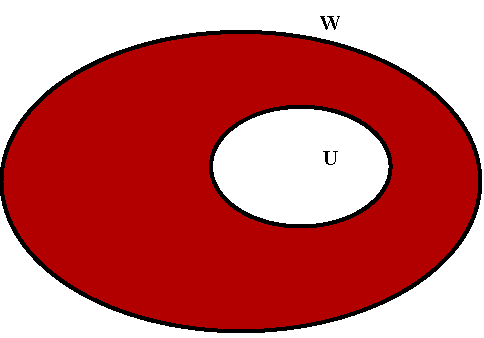
\includegraphics[width=.7\textwidth]{img/exams/2022-02-09/insiemi.pdf}
	\end{figure}
	
	\noindent
	Risulta evidente che se combinando gli elementi di $U$ si ottiene $W$, allora vuol dire che $U$ è un sottoinsieme di $W$. Dunque, per definizione della teoria degli insiemi, l'intersezione tra un insieme e il suo sottoinsieme ritorna l'insieme più grande.\newline
	
	\noindent
	Quindi, applicando la formula di Grassman, la dimensione è:
	\begin{equation*}
		\dim\left(W+U\right) = \dim\left(W\right) + \dim\left(U\right) - \dim\left(W \cap U\right) = 1 + 2 - 1 = 2
	\end{equation*}\newpage

	\subsubsection{Esercizio 2}

	\textcolor{Red3}{\textbf{Esercizio}}\newline
	
	\noindent
	Siano $v_{1} = \begin{pmatrix}
		1 \\
		2 \\
		0
	\end{pmatrix}, v_{2} = \begin{pmatrix}
		1 \\
		0 \\
		5
	\end{pmatrix}$ come nell'esercizio 1 e sia $S$ la matrice con le colonne $v_{1}, v_{2}$ e $v_{3} = \begin{pmatrix}
		2 \\
		2 \\
		0
	\end{pmatrix}$. Si dimostri che $\mathcal{B} = \left\{v_{1}, v_{2}, v_{3}\right\}$ è una base di $\mathbb{R}^{3}$ e si calcoli la matrice inversa $S^{-1}$.\newline
	
	\noindent
	\textcolor{Green4}{\textbf{Soluzione}}\newline
	
	\noindent
	Il sottospazio $\mathcal{B}$ è una base di $\mathbb{R}^{3}$ se $v_{1}, v_{2}, v_{3}$ sono linearmente indipendenti. Quindi, si costruisce una matrice $S$ avente come colonne i vettori del sottospazio:
	\begin{equation*}
		S = \begin{bmatrix}
			1 & 1 & 2 \\
			2 & 0 & 2 \\
			0 & 5 & 0
		\end{bmatrix}
	\end{equation*}
	Per verificare che le colonne siano linearmente indipendenti, si sceglie una delle seguenti opzioni:
	\begin{enumerate}
		\item Il determinante della matrice deve essere diverso da zero;
		
		\item Il rango deve essere uguale al numero di righe;
		
		\item Il sistema aumentato $Ax = 0$ possiede solo la soluzione $x = 0$.
	\end{enumerate}
	Dato che dopo è necessario calcolare la matrice inversa, si opta per seguire la strada del rango. Infatti, il rango corrisponde al numero di colonne dominanti nella forma ridotta. Per ottenere quest'ultima è necessario applicare l'eliminazione di Gauss. Si inizia con la moltiplicazione della prima riga per $-2$ e poi si somma la prima riga con la seconda:
	\begin{equation*}
		S = \begin{bmatrix}
			1 & 1 & 2 \\
			2 & 0 & 2 \\
			0 & 5 & 0
		\end{bmatrix} \xlongrightarrow{E_{2,1}\left(-2\right)} \begin{bmatrix}
			1 & 1 & 2 \\
			0 & -2 & -2 \\
			0 & 5 & 0
		\end{bmatrix}
	\end{equation*}
	Si \textbf{moltiplica la seconda riga per $-\frac{1}{2}$}. Successivamente, si \textbf{moltiplica la seconda riga per $-5$ e poi si somma la seconda riga con la terza}:
	\begin{equation*}
		\begin{bmatrix}
			1 & 1 & 2 \\
			0 & -2 & -2 \\
			0 & 5 & 0
		\end{bmatrix} \xlongrightarrow[E_{3,2}\left(-5\right)]{E_{2}\left(-\frac{1}{2}\right)} \begin{bmatrix}
			1 & 1 & 2 \\
			0 & 1 & 1 \\
			0 & 0 & -5
		\end{bmatrix}
	\end{equation*}
	Si \textbf{moltiplica la terza riga per $-\frac{1}{5}$}:
	\begin{equation*}
		\begin{bmatrix}
			1 & 1 & 2 \\
			0 & 1 & 1 \\
			0 & 0 & -5
		\end{bmatrix} \xlongrightarrow{E_{3}\left(-\frac{1}{5}\right)} \begin{bmatrix}
			1 & 1 & 2 \\
			0 & 1 & 1 \\
			0 & 0 & 1
		\end{bmatrix}
	\end{equation*}
	Dalla forma ridotta è possibile calcolare il rango grazie al numero di colonne dominante. Quindi:
	\begin{equation*}
		\mathrm{rk}\left(S\right) = 3
	\end{equation*}
	Dato che il rango corrisponde al numero di righe della matrice $S$, allora le colonne sono linearmente indipendenti. Questo comporta che il sottospazio $\mathcal{B}$ è una base di $\mathbb{R}^{3}$.\newline
	
	\noindent
	Adesso si calcola la matrice inversa e per farlo si utilizza la matrice aumentata aggiungendo la matrice identità e poi si esegue l'eliminazione di Gauss. Grazie alla forma ridotta calcolata precedentemente si arriva già ad un buon punto:
	\begin{equation*}
		\left[S | I_{3}\right] = \begin{rowequmatbra}{ccc|ccc}
			1 & 1 & 2 & 1 & 0 & 0 \\ [0.3em]
			2 & 0 & 2 & 0 & 1 & 0 \\ [0.3em]
			0 & 5 & 0 & 0 & 0 & 1
		\end{rowequmatbra}
		\xlongrightarrow[E_{3,2}\left(-5\right), E_{3}\left(-\frac{1}{5}\right)]{E_{2,1}\left(-2\right), E_{2}\left(-\frac{1}{2}\right)}
		\begin{rowequmatbra}{ccc|ccc}
			1 & 1 & 2 & 1 & 0 & 0 \\ [0.3em]
			0 & 1 & 1 & 1 & -\frac{1}{2} & 0 \\ [0.3em]
			0 & 0 & 1 & 1 & -\frac{1}{2} & -\frac{1}{5}
		\end{rowequmatbra}
	\end{equation*}
	Si \textbf{moltiplica la terza riga per $-1$ e poi si somma la terza riga con la seconda}. Successivamente si \textbf{moltiplica la terza riga per $-2$ e poi si somma la terza riga con la prima}:
	\begin{equation*}
		\begin{rowequmatbra}{ccc|ccc}
			1 & 1 & 2 & 1 & 0 & 0 \\ [0.3em]
			0 & 1 & 1 & 1 & -\frac{1}{2} & 0 \\ [0.3em]
			0 & 0 & 1 & 1 & -\frac{1}{2} & -\frac{1}{5}
		\end{rowequmatbra}
		\xlongrightarrow[E_{1,3}\left(-2\right)]{E_{2,3}\left(-1\right)}
		\begin{rowequmatbra}{ccc|ccc}
			1 & 1 & 0 & -1 & 1 & \frac{2}{5} \\ [0.3em]
			0 & 1 & 0 &  0 & 0 & \frac{1}{5} \\ [0.3em]
			0 & 0 & 1 &  1 & -\frac{1}{2} & -\frac{1}{5}
		\end{rowequmatbra}
	\end{equation*}
	Si \textbf{moltiplica la seconda riga per $-1$ e poi si somma la seconda riga con la prima}:
	\begin{equation*}
		\begin{rowequmatbra}{ccc|ccc}
			1 & 1 & 0 & -1 & 1 & \frac{2}{5} \\ [0.3em]
			0 & 1 & 0 &  0 & 0 & \frac{1}{5} \\ [0.3em]
			0 & 0 & 1 &  1 & -\frac{1}{2} & -\frac{1}{5}
		\end{rowequmatbra}
		\xlongrightarrow{E_{1,2}\left(-1\right)}
		\begin{rowequmatbra}{ccc|ccc}
			1 & 0 & 0 & -1 & 1 & \frac{1}{5} \\ [0.3em]
			0 & 1 & 0 &  0 & 0 & \frac{1}{5} \\ [0.3em]
			0 & 0 & 1 &  1 & -\frac{1}{2} & -\frac{1}{5}
		\end{rowequmatbra}
	\end{equation*}
	A sinistra è stata ottenuta la matrice identità, dunque a destra si può osservare la matrice invertita:
	\begin{equation*}
		S^{-1} = \begin{rowequmatbra}{ccc}
			-1 & 1 & \frac{1}{5} \\ [0.3em]
			0 & 0 & \frac{1}{5} \\ [0.3em]
			 1 & -\frac{1}{2} & -\frac{1}{5}
		\end{rowequmatbra}
	\end{equation*}\newpage
	
	\subsubsection{Esercizio 3}
	
	\textcolor{Red3}{\textbf{Esercizio}}\newline
	
	\noindent
	Si consideri l'applicazione lineare $f:\mathbb{R}^{3} \rightarrow \mathbb{R}^{3}$, $
	\begin{pmatrix}
		x_{1} \\
		x_{2} \\
		x_{3}
	\end{pmatrix}
	\mapsto
	\begin{pmatrix}
		x_{1} + x_{3} 	\\
		x_{2} + 2x_{3} 	\\
		x_{1} + 2x_{2} + 5x_{3}
	\end{pmatrix}$.
	\begin{enumerate}[label=(\alph*)]
		\item Si trovi la matrice $A$ associata a $f$ rispetto alla base canonica sul dominio e sul codominio. Inoltre si calcolino il rango e il determinante della matrice $A$.
		
		\item Si trovi una base dello spazio nullo di $f$.
		
		\item Si trovi la matrice $B$ associata a $f$ rispetto alla base $\mathcal{B} = \left\{v_{1}, v_{2}, v_{3}\right\}$ dell'esercizio 2 sul domino e sul codominio.
		
		\item Il vettore $u = 2v_{1} + v_{2} - v_{3}$ appartiene all'immagine di $f$? Se sì, si determini l'insieme $L$ dato da tutti i vettori $v \in \mathbb{R}^{3}$ tali che $f\left(v\right) = u$.
	\end{enumerate}
	
	\noindent
	\textcolor{Green4}{\textbf{Soluzione caso \emph{a}}}\newline
	
	\noindent
	La matrice $A$ associata a $f$ rispetto alla base canonica ha come colonne $f\left(e_{1}\right), f\left(e_{2}\right), f\left(e_{3}\right)$. Quindi, si scrive la matrice $A$ come la composizione di $f$:
	\begin{equation*}
		A = \left( f\left(\begin{bmatrix}
			1 \\
			0 \\
			0
		\end{bmatrix}\right) \: f\left(\begin{bmatrix}
			0 \\
			1 \\
			0
		\end{bmatrix}\right) \: f\left(\begin{bmatrix}
			0 \\
			0 \\
			1
		\end{bmatrix}\right)\right)
	\end{equation*}
	Quindi, per ogni colonna si calcola la colonna risultante. Per farlo, si sostituiscono i valori di ogni colonna nell'applicazione lineare $\begin{pmatrix}
		x_{1} + x_{3} 	\\
		x_{2} + 2x_{3} 	\\
		x_{1} + 2x_{2} + 5x_{3}
	\end{pmatrix}$:
	\begin{equation*}
		\begin{array}{lllll}
			f\left(\begin{bmatrix}
				1 \\
				0 \\
				0
			\end{bmatrix}\right) & = & \begin{pmatrix}
				1 + 0 	\\
				0 + 2 \cdot 0 	\\
				1 + 2 \cdot 0 + 5 \cdot 0
			\end{pmatrix} & = & \begin{pmatrix}
				1 \\
				0 \\
				1
			\end{pmatrix} \\
			%
			\\
			%
			f\left(\begin{bmatrix}
				0 \\
				1 \\
				0
			\end{bmatrix}\right) & = & \begin{pmatrix}
				0 + 0 	\\
				1 + 2 \cdot 0 	\\
				0 + 2 \cdot 1 + 5 \cdot 0
			\end{pmatrix} & = & \begin{pmatrix}
				0 \\
				1 \\
				2
			\end{pmatrix} \\
			%
			\\
			%
			f\left(\begin{bmatrix}
				0 \\
				0 \\
				1
			\end{bmatrix}\right) & = & \begin{pmatrix}
				0 + 1 	\\
				0 + 2 \cdot 1 	\\
				0 + 2 \cdot 0 + 5 \cdot 1
			\end{pmatrix} & = & \begin{pmatrix}
				1 \\
				2 \\
				5
			\end{pmatrix}
		\end{array}
	\end{equation*}
	La matrice risultante si ottiene combinando tutti i vettori:
	\begin{equation*}
		A = \begin{bmatrix}
			1 & 0 & 1 \\
			0 & 1 & 2 \\
			1 & 2 & 5
		\end{bmatrix}
	\end{equation*}\newpage
	
	\noindent
	Inoltre l'esercizio richiede sia il determinante che il rango. Per quest'ultimo si esegue l'eliminazione di Gauss e si ottiene la forma ridotta. Quindi, si \textbf{moltiplica la prima riga per $-1$}:
	\begin{equation*}
		\begin{bmatrix}
			1 & 0 & 1 \\
			0 & 1 & 2 \\
			1 & 2 & 5
		\end{bmatrix}
		\xlongrightarrow{E_{3,1}\left(-1\right)}
		\begin{bmatrix}
			1 & 0 & 1 \\
			0 & 1 & 2 \\
			0 & 2 & 4
		\end{bmatrix}
	\end{equation*}
	Si \textbf{moltiplica la seconda riga per $-2$ e poi si somma la seconda riga con la terza}:
	\begin{equation*}
		\begin{bmatrix}
			1 & 0 & 1 \\
			0 & 1 & 2 \\
			0 & 2 & 4
		\end{bmatrix}
		\xlongrightarrow{E_{3,2}\left(-2\right)}
		\begin{bmatrix}
			1 & 0 & 1 \\
			0 & 1 & 2 \\
			0 & 0 & 0
		\end{bmatrix}
	\end{equation*}
	Data la forma ridotta, il rango corrisponde al numero di colonne dominanti, cioè $2$:
	\begin{equation*}
		\mathrm{rk}\left(A\right) = 2
	\end{equation*}
	Infine, il determinante viene calcolato (come calcolarlo, paragrafo \ref{Determinante}) tenendo in considerazione anche le operazioni di EG eseguite. In questo caso, le operazioni sono identiche e non hanno influenza sul determinante poiché sono le uniche operazioni elementari ininfluenti. Quindi, il determinante viene calcolato banalmente moltiplicando tra di loro i coefficienti posti sulla diagonale principale:
	\begin{equation*}
		\det\left(A\right) = \det\left(U\right) = 1 \cdot 1 \cdot 0 = 0
	\end{equation*}
	Dove $U$ è la forma ridotta ottenuta con l'eliminazione di Gauss.\newpage
	
	\noindent
	\textcolor{Green4}{\textbf{Soluzione caso \emph{b}}}\newline
	
	\noindent
	Lo spazio nullo di $f$ non è altro che:
	\begin{equation*}
		N\left(f\right) = \left\{v \in \mathbb{R}^{3} \: \left| f\left(v\right) = 0 \right.\right\} = \left\{v \in \mathbb{R}^{3} \: \left| Av = 0 \right.\right\}
	\end{equation*}
	Ovvero tutti quei vettori appartenenti all'insieme $\mathbb{R}^{3}$ tale per cui data la matrice associata e moltiplicata per il vettore, il risultato è zero. Quindi, gli elementi dello spazio nullo $N\left(f\right)$ sono le soluzioni:
	\begin{equation*}
		\begin{cases}
			x_{1} + x_{3} = 0 	\\
			x_{2} + 2x_{3} = 0 	\\
			x_{1} + 2x_{2} + 5x_{3} = 0
		\end{cases}
	\end{equation*}
	Andando a sostituire le variabili $x_{1} = x, x_{2} = y, x_{3} = z$:
	\begin{equation*}
		\begin{cases}
			x + z = 0 	\\
			y + 2z = 0 	\\
			x + 2y + 5z = 0
		\end{cases}
	\end{equation*}
	Grazie all'applicazione dell'eliminazione di Gauss eseguita al passo \emph{a}, si è già in possesso della forma ridotta della matrice associata $A$:
	\begin{equation*}
		\begin{bmatrix}
			1 & 0 & 1 \\
			0 & 1 & 2 \\
			0 & 0 & 0
		\end{bmatrix}
	\end{equation*}
	Da essa si ricava il sistema da porre uguale a zero:
	\begin{equation*}
		\begin{cases}
			x + z = 0 	\\
			y + 2z = 0
		\end{cases}
	\end{equation*}
	Adesso si risolve banalmente il sistema:
	\begin{equation*}
		\begin{cases}
			x + z = 0 	\\
			y + 2z = 0
		\end{cases} \Rightarrow \begin{cases}
			x = -z \\
			y = -2z
		\end{cases}
	\end{equation*}
	Quindi, si ottiene il vettore risultante composto come:
	\begin{equation*}
		\begin{bmatrix}
			-z \\
			-2z \\
			z
		\end{bmatrix}
	\end{equation*}
	E lo spazio nullo dunque sarà formato:
	\begin{equation*}
		N\left(f\right) = \left\{\left. \begin{bmatrix}
			-z \\
			-2z \\
			z
		\end{bmatrix} \: \right| \: z \in \mathbb{R}\right\}
	\end{equation*}
	Dove il vettore $\left\langle \begin{pmatrix}
		-1 \\
		-2 \\
		1
	\end{pmatrix}\right\rangle$ è una base dello spazio nullo.\newpage

	\noindent
	\textcolor{Green4}{\textbf{Soluzione caso \emph{c}}}\newline
	
	\noindent
	Nell'esercizio 2, la base era:
	\begin{equation*}
		\mathcal{B} = \left\{v_{1}, v_{2}, v_{3}\right\} = \left\{
		\begin{pmatrix}
			1 \\
			2 \\
			0
		\end{pmatrix},
		\begin{pmatrix}
			1 \\
			0 \\
			5
		\end{pmatrix},
		\begin{pmatrix}
			2 \\
			2 \\
			0
		\end{pmatrix}
		\right\}
	\end{equation*}
	Per trovare la matrice $B$ associata a $f$ rispetto alla base $\mathcal{B}$, è necessario prima di tutto calcolare l'applicazione lineare. Per definizione del teorema, la matrice $B$ è composta dalle colonne:
	\begin{equation*}
		B = \begin{bmatrix}
			C_{B}\left(f\left(v_{1}\right)\right) & C_{B}\left(f\left(v_{2}\right)\right) & C_{B}\left(f\left(v_{3}\right)\right)
		\end{bmatrix}
	\end{equation*}
	Dove $C_{B}$ rappresenta l'applicazione lineare. Rispetto al caso \emph{a}, in questo caso è necessario qualche passaggio in più. Infatti, nel primo caso la base canonica è immediata da scrivere. Mentre in questo caso è necessario calcolare l'applicazione lineare:
	\begin{equation*}
		C_{B} : \mathbb{R}^{3} \longrightarrow \mathbb{R}^{3}
	\end{equation*}
	Data l'applicazione lineare in $\mathbb{R}^{3}$, si scrive l'applicazione lineare corrispettiva:
	\begin{equation*}
		\begin{bmatrix}
			x \\
			y \\
			z
		\end{bmatrix} = \alpha \begin{bmatrix}
			1 \\
			2 \\
			0
		\end{bmatrix} + \beta \begin{bmatrix}
			1 \\
			0 \\
			5
		\end{bmatrix} + \gamma \begin{bmatrix}
			2 \\
			2 \\
			0
		\end{bmatrix} = \begin{bmatrix}
			1 & 1 & 2 \\
			2 & 0 & 2 \\
			0 & 5 & 0
		\end{bmatrix} \begin{bmatrix}
			\alpha \\
			\beta \\
			\gamma
		\end{bmatrix}
	\end{equation*}
	Quindi, l'applicazione lineare corrispettiva è:
	\begin{equation*}
		C_{B}\left(\begin{bmatrix}
			x \\
			y \\
			z
		\end{bmatrix}\right) = \begin{bmatrix}
			\alpha \\
			\beta \\
			\gamma
		\end{bmatrix}
	\end{equation*}
	Per trovare le incognite $\alpha, \beta, \gamma$ si considera il sistema lineare:
	\begin{equation*}
		\begin{bmatrix}
			1 & 1 & 2 \\
			2 & 0 & 2 \\
			0 & 5 & 0
		\end{bmatrix} \begin{bmatrix}
			\alpha \\
			\beta \\
			\gamma
		\end{bmatrix} = \begin{bmatrix}
			x \\
			y \\
			z
		\end{bmatrix}
	\end{equation*}
	Quindi, si può applicare l'eliminazione di Gauss, considerando la matrice aumentata:
	\begin{equation*}
		\begin{rowequmatbra}{ccc|c}
			1 & 1 & 2 & x \\
			2 & 0 & 2 & y \\
			0 & 5 & 0 & z
		\end{rowequmatbra}
	\end{equation*}
	Si \textbf{moltiplica la prima riga per $-2$ e poi si somma la prima riga con la seconda}:
	\begin{equation*}
		\begin{rowequmatbra}{ccc|c}
			1 & 1 & 2 & x \\
			2 & 0 & 2 & y \\
			0 & 5 & 0 & z
		\end{rowequmatbra}
		\xlongrightarrow{E_{2,1}\left(-2\right)}
		\begin{rowequmatbra}{ccc|c}
			1 & 1 & 2 & x \\
			0 & -2 & -2 & y-2x \\
			0 & 5 & 0 & z
		\end{rowequmatbra}
	\end{equation*}
	Si \textbf{moltiplica la seconda riga per $-\frac{1}{2}$}:
	\begin{equation*}
		\begin{rowequmatbra}{ccc|c}
			1 & 1 & 2 & x \\ [0.3em]
			0 & -2 & -2 & y-2x \\ [0.3em]
			0 & 5 & 0 & z
		\end{rowequmatbra}
		\xlongrightarrow{E_{2}\left(-\frac{1}{2}\right)}
		\begin{rowequmatbra}{ccc|c}
			1 & 1 & 2 & x \\ [0.3em]
			0 & 1 & 1 & \frac{2x-y}{2} \\ [0.3em]
			0 & 5 & 0 & z
		\end{rowequmatbra}
	\end{equation*}
	Si \textbf{moltiplica la seconda riga per $-5$ e poi si somma la seconda riga con la terza}:
	\begin{equation*}
		\begin{rowequmatbra}{ccc|c}
			1 & 1 & 2 & x \\ [0.3em]
			0 & 1 & 1 & \frac{2x-y}{2} \\ [0.3em]
			0 & 5 & 0 & z
		\end{rowequmatbra}
		\xlongrightarrow{E_{3,2}\left(-5\right)}
		\begin{rowequmatbra}{ccc|c}
			1 & 1 & 2 & x \\ [0.3em]
			0 & 1 & 1 & \frac{2x-y}{2} \\ [0.3em]
			0 & 0 & -5 & z-5\left(\frac{2x-y}{2}\right)
		\end{rowequmatbra}
	\end{equation*}
	Si \textbf{moltiplica la terza riga per $-\frac{1}{5}$}:
	\begin{equation*}
		\begin{rowequmatbra}{ccc|c}
			1 & 1 & 2 & x \\ [0.3em]
			0 & 1 & 1 & \frac{2x-y}{2} \\ [0.3em]
			0 & 0 & -5 & z-5\left(\frac{2x-y}{2}\right)
		\end{rowequmatbra}
		\xlongrightarrow{E_{3}\left(-\frac{1}{5}\right)}
		\begin{rowequmatbra}{ccc|c}
			1 & 1 & 2 & x \\ [0.3em]
			0 & 1 & 1 & \frac{2x-y}{2} \\ [0.3em]
			0 & 0 & 1 & \left(\frac{10x-5y-2z}{10}\right)
		\end{rowequmatbra}
	\end{equation*}
	La forma ridotta è stata ottenuta, adesso si scrive il sistema lineare dipendente:
	\begin{equation*}
		\begin{cases}
			\alpha = x - \beta - 2\gamma \\
			\\
			\beta = \dfrac{2x-y}{2} - \left(\dfrac{10x-5y-2z}{10}\right) \\
			\\
			\gamma = \dfrac{10x-5y-2z}{10}
		\end{cases} \Longrightarrow
		\begin{cases}
			\alpha = x - \dfrac{z}{5} - \left(\dfrac{10x-5y-2z}{5}\right) = \dfrac{-5x+5y+z}{5}\\
			\\
			\beta = \dfrac{10x-5y-10x+5y+2z}{10} = \dfrac{z}{5} \\
			\\
			\gamma = \dfrac{10x-5y-2z}{10}
		\end{cases}
	\end{equation*}
	Grazie alle soluzioni è possibile scrivere il vettore soluzione come:
	\begin{equation*}
		C_{B} = \left(\begin{bmatrix}
			x \\
			y \\
			z
		\end{bmatrix}\right) = \begin{rowequmatbra}{c}
			\frac{-5x+5y+z}{5} \\ [0.3em]
			\frac{z}{5} \\ [0.3em]
			\frac{10x-5y-2z}{10}
		\end{rowequmatbra} = \begin{rowequmatbra}{c}
			-x+y+\frac{z}{5} \\ [0.3em]
			\frac{z}{5} \\ [0.3em]
			x - \frac{y}{2} - \frac{z}{5}
		\end{rowequmatbra}
	\end{equation*}
	Adesso si eseguono le sostituzioni iniziali dell'applicazione lineare. Prima di tutto si sostituiscono i valori dei vettori $v_{1}, v_{2}, v_{3}$ nell'applicazione lineare $f$:
	\begin{equation*}
		\begin{array}{lllllll}
			C_{B}\left(f\left(v_{1}\right)\right) & = & C_{B}\left(f\left(\begin{bmatrix}
				1 \\
				2 \\
				0
			\end{bmatrix}\right)\right) & = & \begin{bmatrix}
				1 + 0 \\
				2 + 2 \cdot 0 	\\
				1 + 2 \cdot 2 + 5 \cdot 0
			\end{bmatrix} & = & C_{B}\left(\begin{bmatrix}
				1 \\
				2 \\
				5
			\end{bmatrix}\right) \\
			\\
			C_{B}\left(f\left(v_{2}\right)\right) & = & C_{B}\left(f\left(\begin{bmatrix}
				1 \\
				0 \\
				5
			\end{bmatrix}\right)\right) & = & \begin{bmatrix}
				1 + 5 	\\
				0 + 2 \cdot 5 	\\
				1 + 2 \cdot 0 + 5 \cdot 5
			\end{bmatrix} & = & C_{B}\left(\begin{bmatrix}
				6 \\
				0 \\
				26
			\end{bmatrix}\right) \\
			\\
			C_{B}\left(f\left(v_{3}\right)\right) & = & C_{B}\left(f\left(\begin{bmatrix}
				2 \\
				2 \\
				0
			\end{bmatrix}\right)\right) & = & \begin{bmatrix}
				2 + 0 	\\
				2 + 2 \cdot 0 	\\
				2 + 2 \cdot 2 + 5 \cdot 0
			\end{bmatrix} & = & C_{B}\left(\begin{bmatrix}
				2 \\
				2 \\
				6
			\end{bmatrix}\right)
		\end{array}
	\end{equation*}\newpage
	
	\noindent
	Poi si inseriscono i valori nell'applicazione lineare $C_{B}$, ovvero nel vettore soluzione ottenuto dal sistema:
	\begin{equation*}
		\begin{array}{lllll}
			C_{B}\left(\begin{bmatrix}
				1 \\
				2 \\
				5
			\end{bmatrix}\right) & = & \begin{bmatrix}
				-1 +2 +1 \\
				1 \\
				1 -1 -1
			\end{bmatrix} & = & \begin{bmatrix}
				2 \\
				1 \\
				-1
			\end{bmatrix} \\
			\\
			C_{B}\left(\begin{bmatrix}
				6 \\
				10 \\
				26
			\end{bmatrix}\right) & = & \begin{rowequmatbra}{c}
				-6 +10 +\frac{26}{5} \\ [0.3em]
				\frac{26}{5} \\ [0.3em]
				6 -5 -\frac{26}{5}
			\end{rowequmatbra} & = & \begin{rowequmatbra}{c}
				\frac{46}{5} \\ [0.3em]
				\frac{26}{5} \\ [0.3em]
				-\frac{21}{5}
			\end{rowequmatbra} \\
			\\
			C_{B}\left(\begin{bmatrix}
				2 \\
				2 \\
				6
			\end{bmatrix}\right) & = & \begin{rowequmatbra}{c}
				-2 +2 +\frac{6}{5} \\ [0.3em]
				\frac{6}{5} \\ [0.3em]
				2 -1 -\frac{6}{5}
			\end{rowequmatbra} & = & \begin{rowequmatbra}{c}
				\frac{6}{5} \\ [0.3em]
				\frac{6}{5} \\ [0.3em]
				-\frac{1}{5}
			\end{rowequmatbra}
		\end{array}
	\end{equation*}
	Si ricostruisce la matrice $B$:
	\begin{equation*}
		B = \begin{rowequmatbra}{ccc}
			2 	& \frac{46}{5}	& \frac{6}{5} \\ [0.3em]
			1 	& \frac{26}{5}	& \frac{6}{5} \\ [0.3em]
			-1	& -\frac{21}{5}	& -\frac{1}{5}
		\end{rowequmatbra} = \dfrac{1}{5} \begin{rowequmatbra}{ccc}
			10 	& 46	& 6 \\ [0.3em]
			5	& 26	& 6 \\ [0.3em]
			-5	& -21	& -1
		\end{rowequmatbra}
	\end{equation*}\newpage
	
	\noindent
	\textcolor{Green4}{\textbf{Soluzione caso \emph{d}}}\newline
	
	\noindent
	Il vettore $u$ appartiene all'immagine di $f$ se e solo se esiste un vettore $v \in \mathbb{R}^{3}$ tale per cui $f\left(v\right) = u$. Ovvero se l'applicazione lineare su $f$ restituisce $u$. Quindi, si sostituiscono i vettori nell'equazione di $u$:
	\begin{equation*}
		u = 2\begin{bmatrix}
			1 \\
			2 \\
			0
		\end{bmatrix} + \begin{bmatrix}
			1 \\
			0 \\
			5
		\end{bmatrix} - \begin{bmatrix}
			2 \\
			2 \\
			0
		\end{bmatrix} = \begin{bmatrix}
			1 \\
			2 \\
			5	
		\end{bmatrix}
	\end{equation*}
	Per dimostrare che $u$ è un'immagine di $f$, si pone l'uguaglianza dell'applicazione lineare di $f$ con il vettore $u$:
	\begin{equation*}
		\begin{cases}
			x_{1} + x_{3} = 1 \\
			x_{2} + 2x_{3} = 2 \\
			x_{1} + 2x_{2} + 5x_{3} = 5
		\end{cases}
	\end{equation*}
	Per risolvere il sistema si applica l'EG tramite la matrice aumentata. La prima operazione è la \textbf{moltiplicazione della prima riga per $-1$ e poi si somma la prima riga con la terza}:
	\begin{equation*}
		\begin{rowequmatbra}{ccc|c}
			1 & 0 & 1 & 1 \\
			0 & 1 & 2 & 2 \\
			1 & 2 & 5 & 5
		\end{rowequmatbra}
		\xlongrightarrow{E_{3,1}\left(-1\right)}
		\begin{rowequmatbra}{ccc|c}
			1 & 0 & 1 & 1 \\
			0 & 1 & 2 & 2 \\
			0 & 2 & 4 & 4
		\end{rowequmatbra}
	\end{equation*}
	Si \textbf{moltiplica la seconda riga per $-2$ e poi si somma la seconda riga con la terza}:
	\begin{equation*}
		\begin{rowequmatbra}{ccc|c}
			1 & 0 & 1 & 1 \\
			0 & 1 & 2 & 2 \\
			0 & 2 & 4 & 4
		\end{rowequmatbra}
		\xlongrightarrow{E_{3,2}\left(-2\right)}
		\begin{rowequmatbra}{ccc|c}
			1 & 0 & 1 & 1 \\
			0 & 1 & 2 & 2 \\
			0 & 0 & 0 & 0
		\end{rowequmatbra}
	\end{equation*}
	Si ottiene la forma ridotta e si riporta i coefficienti nel sistema lineare:
	\begin{equation*}
		\begin{cases}
			x_{1} + x_{3} = 1 \\
			x_{2} + 2x_{3} = 2
		\end{cases} \Longrightarrow \begin{cases}
			x_{1} = 1 - x_{3} \\
			x_{2} = 2 - 2x_{3}
		\end{cases}
	\end{equation*}
	Il vettore risultante dipende dal parametro $x_{3}$:
	\begin{equation*}
		\begin{bmatrix}
			1-x_{3} \\
			2-2x_{3} \\
			x_{3}
		\end{bmatrix}
	\end{equation*}
	Per verificare che il vettore $u$ appartenga all'immagine di $f$, si prova a dare un valore a $x_{3}$ e verificare. Quindi, si assegna $x_{3} = 1$, il vettore diventa:
	\begin{equation*}
		v = \begin{bmatrix}
			0 \\
			0 \\
			1
		\end{bmatrix}
	\end{equation*}
	E applicando il vettore all'applicazione lineare $f\left(v\right)$:
	\begin{equation*}
		f\left(v\right) = f\left(\begin{bmatrix}
			0 \\
			0 \\
			1
		\end{bmatrix}\right) = \begin{bmatrix}
			0 + 1 \\
			0 + 2 \cdot 1 \\
			0 + 2 \cdot 0 + 5 \cdot 1
		\end{bmatrix} = \begin{bmatrix}
			1 \\
			2 \\
			5
		\end{bmatrix} = u \textcolor{Green4}{\textbf{ \checkmark Verificato}}
	\end{equation*}
	Dato che il vettore $u$ appartiene all'immagine di $f$, si deve determinare l'insieme $L$. Quest'ultimo ha la caratteristica di contenere tutti i vettori tali per cui la loro applicazione lineare $f$ sia uguale a $u$. Grazie alla definizione di un teorema, è noto che l'insieme delle soluzioni è composto dalla somma del vettore soluzione e un vettore appartenente all'insieme nullo:
	\begin{equation*}
		L = \left\{x + w \: | \: w \in N\left(A\right)\right\}
	\end{equation*}
	Dato che una base dello spazio nullo era già stato trovato al punto \emph{b}, si riutilizza quella soluzione:
	\begin{equation*}
		L = \left\{\left. v + \begin{bmatrix}
			-z \\
			-2z \\
			z
		\end{bmatrix} \right| z \in \mathbb{R}\right\}
	\end{equation*}\newpage

	\subsubsection{Esercizio 4}
	
	\textcolor{Red3}{\textbf{Esercizio}}\newline
	
	\noindent
	Vero o falso? Si motivi la risposta!
	
	\begin{enumerate}
		\item Se $\lambda$ è un autovalore di una matrice $A$, allora $\lambda^{2}$ è autovalore della matrice $A^{2}$.
		
		\item La matrice $\begin{bmatrix}
				0 & 0 & 1 \\
				0 & 4 & 0
			\end{bmatrix}$ possiede un'inversa sinistra.
	\end{enumerate}
	
	\noindent
	\textcolor{Green4}{\textbf{Soluzione caso 1}}\newline
	
	\noindent
	La risposta è vero. Infatti, $\lambda$ è autovalore di $A$ se esiste un vettore $v \in V$ tale che $Av = \lambda v$. Quindi:
	\begin{equation*}
		A^{2}v = A\left(Av\right) = A\left(\lambda v\right) = \lambda{Av} = \lambda^{2}v
	\end{equation*}
	Dunque $\lambda^{2}$ è autovalore di $A$.\newline
	
	\noindent
	\textcolor{Green4}{\textbf{Soluzione caso 2}}\newline
	
	\noindent
	La risposta è falso. Infatti, la matrice non possiede un'inversa sinistra poiché il numero di righe non è maggiore o uguale al numero di colonne.
\end{document}